\documentclass[12pt,ignorenonframetext,aspectratio=169]{beamer}
\setbeamertemplate{caption}[numbered]
\setbeamertemplate{caption label separator}{: }
\setbeamercolor{caption name}{fg=normal text.fg}
\beamertemplatenavigationsymbolsempty
\usepackage{lmodern}

\DeclareMathOperator*{\argmin}{arg\,min}
\DeclareMathOperator*{\argmax}{arg\,max}
\newcommand{\code}[1]{\texttt{#1}}
\newcommand{\pkg}[1]{\textbf{#1}}

\usepackage{amssymb,amsmath}
\usepackage{ifxetex,ifluatex}
\usepackage{fixltx2e} % provides \textsubscript
\ifnum 0\ifxetex 1\fi\ifluatex 1\fi=0 % if pdftex
  \usepackage[T1]{fontenc}
  \usepackage[utf8]{inputenc}
\else % if luatex or xelatex
  \ifxetex
    \usepackage{mathspec}
  \else
    \usepackage{fontspec}
  \fi
  \defaultfontfeatures{Ligatures=TeX,Scale=MatchLowercase}
\fi
\usetheme[]{metropolis}
\usefonttheme{professionalfonts}
% use upquote if available, for straight quotes in verbatim environments
\IfFileExists{upquote.sty}{\usepackage{upquote}}{}
% use microtype if available
\IfFileExists{microtype.sty}{%
\usepackage{microtype}
\UseMicrotypeSet[protrusion]{basicmath} % disable protrusion for tt fonts
}{}
\newif\ifbibliography
\hypersetup{
            pdftitle={gendered-Language-in-digital-spaces},
            pdfauthor={Taylor Arnold},
            pdfborder={0 0 0},
            breaklinks=true}
\urlstyle{same}  % don't use monospace font for urls
\usepackage{color}
\usepackage{fancyvrb}
\newcommand{\VerbBar}{|}
\newcommand{\VERB}{\Verb[commandchars=\\\{\}]}
\DefineVerbatimEnvironment{Highlighting}{Verbatim}{commandchars=\\\{\}}
% Add ',fontsize=\small' for more characters per line
\usepackage{framed}
\definecolor{shadecolor}{RGB}{248,248,248}
\newenvironment{Shaded}{\begin{snugshade}}{\end{snugshade}}
\newcommand{\KeywordTok}[1]{\textcolor[rgb]{0.13,0.29,0.53}{\textbf{#1}}}
\newcommand{\DataTypeTok}[1]{\textcolor[rgb]{0.13,0.29,0.53}{#1}}
\newcommand{\DecValTok}[1]{\textcolor[rgb]{0.00,0.00,0.81}{#1}}
\newcommand{\BaseNTok}[1]{\textcolor[rgb]{0.00,0.00,0.81}{#1}}
\newcommand{\FloatTok}[1]{\textcolor[rgb]{0.00,0.00,0.81}{#1}}
\newcommand{\ConstantTok}[1]{\textcolor[rgb]{0.00,0.00,0.00}{#1}}
\newcommand{\CharTok}[1]{\textcolor[rgb]{0.31,0.60,0.02}{#1}}
\newcommand{\SpecialCharTok}[1]{\textcolor[rgb]{0.00,0.00,0.00}{#1}}
\newcommand{\StringTok}[1]{\textcolor[rgb]{0.31,0.60,0.02}{#1}}
\newcommand{\VerbatimStringTok}[1]{\textcolor[rgb]{0.31,0.60,0.02}{#1}}
\newcommand{\SpecialStringTok}[1]{\textcolor[rgb]{0.31,0.60,0.02}{#1}}
\newcommand{\ImportTok}[1]{#1}
\newcommand{\CommentTok}[1]{\textcolor[rgb]{0.56,0.35,0.01}{\textit{#1}}}
\newcommand{\DocumentationTok}[1]{\textcolor[rgb]{0.56,0.35,0.01}{\textbf{\textit{#1}}}}
\newcommand{\AnnotationTok}[1]{\textcolor[rgb]{0.56,0.35,0.01}{\textbf{\textit{#1}}}}
\newcommand{\CommentVarTok}[1]{\textcolor[rgb]{0.56,0.35,0.01}{\textbf{\textit{#1}}}}
\newcommand{\OtherTok}[1]{\textcolor[rgb]{0.56,0.35,0.01}{#1}}
\newcommand{\FunctionTok}[1]{\textcolor[rgb]{0.00,0.00,0.00}{#1}}
\newcommand{\VariableTok}[1]{\textcolor[rgb]{0.00,0.00,0.00}{#1}}
\newcommand{\ControlFlowTok}[1]{\textcolor[rgb]{0.13,0.29,0.53}{\textbf{#1}}}
\newcommand{\OperatorTok}[1]{\textcolor[rgb]{0.81,0.36,0.00}{\textbf{#1}}}
\newcommand{\BuiltInTok}[1]{#1}
\newcommand{\ExtensionTok}[1]{#1}
\newcommand{\PreprocessorTok}[1]{\textcolor[rgb]{0.56,0.35,0.01}{\textit{#1}}}
\newcommand{\AttributeTok}[1]{\textcolor[rgb]{0.77,0.63,0.00}{#1}}
\newcommand{\RegionMarkerTok}[1]{#1}
\newcommand{\InformationTok}[1]{\textcolor[rgb]{0.56,0.35,0.01}{\textbf{\textit{#1}}}}
\newcommand{\WarningTok}[1]{\textcolor[rgb]{0.56,0.35,0.01}{\textbf{\textit{#1}}}}
\newcommand{\AlertTok}[1]{\textcolor[rgb]{0.94,0.16,0.16}{#1}}
\newcommand{\ErrorTok}[1]{\textcolor[rgb]{0.64,0.00,0.00}{\textbf{#1}}}
\newcommand{\NormalTok}[1]{#1}
\usepackage{graphicx,grffile}
\makeatletter
\def\maxwidth{\ifdim\Gin@nat@width>\linewidth\linewidth\else\Gin@nat@width\fi}
\def\maxheight{\ifdim\Gin@nat@height>\textheight0.8\textheight\else\Gin@nat@height\fi}
\makeatother
% Scale images if necessary, so that they will not overflow the page
% margins by default, and it is still possible to overwrite the defaults
% using explicit options in \includegraphics[width, height, ...]{}
\setkeys{Gin}{width=\maxwidth,height=\maxheight,keepaspectratio}

\usepackage{graphicx}
\usepackage{libertine}
\usepackage{color}
\usepackage{amssymb}
\usepackage{multirow}
\usepackage{fancyvrb}
\usepackage{listings}
\usepackage{xcolor}

\lstset{
  basicstyle=\ttfamily,
  escapeinside=||
}

\definecolor{solarized@base03}{HTML}{002B36}
\definecolor{solarized@base02}{HTML}{073642}
\definecolor{solarized@base01}{HTML}{586e75}
\definecolor{solarized@base00}{HTML}{657b83}
\definecolor{solarized@base0}{HTML}{839496}
\definecolor{solarized@base1}{HTML}{93a1a1}
\definecolor{solarized@base2}{HTML}{EEE8D5}
\definecolor{solarized@base3}{HTML}{FDF6E3}
\definecolor{solarized@yellow}{HTML}{B58900}
\definecolor{solarized@orange}{HTML}{CB4B16}
\definecolor{solarized@red}{HTML}{DC322F}
\definecolor{solarized@magenta}{HTML}{D33682}
\definecolor{solarized@violet}{HTML}{6C71C4}
\definecolor{solarized@blue}{HTML}{268BD2}
\definecolor{solarized@cyan}{HTML}{2AA198}
\definecolor{solarized@green}{HTML}{859900}
\definecolor{yaleblue}{HTML}{0E4C92}

\newcommand{\yellow}[1]{\textcolor{solarized@yellow}{#1}}
\newcommand{\orange}[1]{\textcolor{solarized@orange}{#1}}
\newcommand{\red}[1]{\textcolor{solarized@red}{#1}}
\newcommand{\magenta}[1]{\textcolor{solarized@magenta}{#1}}
\newcommand{\violet}[1]{\textcolor{solarized@violet}{#1}}
\newcommand{\blue}[1]{\textcolor{solarized@blue}{#1}}
\newcommand{\cyan}[1]{\textcolor{solarized@cyan}{#1}}
\newcommand{\green}[1]{\textcolor{solarized@green}{#1}}
\newcommand{\yblue}[1]{\textcolor{yaleblue}{#1}}
\newcommand{\base}[1]{\textcolor{solarized@base01}{#1}}

% Prevent slide breaks in the middle of a paragraph:
\widowpenalties 1 10000
\raggedbottom

\AtBeginPart{
  \let\insertpartnumber\relax
  \let\partname\relax
  \frame{\partpage}
}
\AtBeginSection{
  \ifbibliography
  \else
    \let\insertsectionnumber\relax
    \let\sectionname\relax
    \frame{\sectionpage}
  \fi
}
\AtBeginSubsection{
  \let\insertsubsectionnumber\relax
  \let\subsectionname\relax
  \frame{\subsectionpage}
}

\setlength{\parindent}{0pt}
\setlength{\parskip}{6pt plus 2pt minus 1pt}
\setlength{\emergencystretch}{3em}  % prevent overfull lines
\providecommand{\tightlist}{%
  \setlength{\itemsep}{0pt}\setlength{\parskip}{0pt}}
\setcounter{secnumdepth}{0}

\title{Enriching Historic Photography with Structured Data
using Image Region Segmentation}
\author{Taylor Arnold and Lauren Tilton}
\date{25-26 May 2020}

% Begin changes
\setbeamertemplate{itemize items}[default]
\setbeamercolor*{item}{fg=black}
\author % (optional, for multiple authors)
{Taylor~Arnold$^{1}$ and Lauren~Tilton$^{2}$}

\institute[] % (optional)
{
  $^{1}$ Assistant Professor of Statistics and Linguistics\\
  University of Richmond\\
  \texttt{statsmaths.github.io}\\

  $^{2}$ Assistant Professor of Digital Humanities\\
  University of Richmond\\
  \texttt{laurentilon.com}\\

}
% End changes

\setbeamertemplate{footline}[text line]{%
  \parbox{\linewidth}{\vspace*{-8pt}Taylor Arnold (@statsmaths) and Lauren Tilton (@nolauren)  \hfill\insertpagenumber}}

\begin{document}
\bibliographystyle{plainnat}

%%%%%%%%%%%%%%%%%%%%%%%%%%%%%%%%%%%

\frame{\titlepage}

% %%%%%%%%%%%%%%%%%%%%%%%%%%%%%%%%%%%%%%%%%%%%%%%%%%%
% \section{Outline}
%
% %%%%%%%%%%%%%%%%%%%%%%%%%%%%%%%%%%%%%%%%%%%%%%%%%%%
% \begin{frame}{}
%
% \begin{itemize}
% \item \orange{Introduction}: what motivates our work
% \item \orange{Data}: description of our example corpus
% \item \orange{Other methods}: overview of prior approaches
% \item \orange{Image region segmentation}: recent computer vision task
% \item \orange{Structured data}: our approach
% \item \orange{Evaluation}: qualitative and quantitative assessment
% \item \orange{Conclusions}
% \end{itemize}
%
% \end{frame}

%%%%%%%%%%%%%%%%%%%%%%%%%%%%%%%%%%%%%%%%%%%%%%%%%%%
\section{Introduction}

%%%%%%%%%%%%%%%%%%%%%%%%%%%%%%%%%%%%%%%%%%%%%%%%%%%
\begin{frame}{}

\begin{itemize}
\item \blue{Guiding question}: How can we increase discovery and access of digitied
photographic collections through structured data and the semantic web. \pause
\item \blue{Challenge}: Lack of structured linguistic descriptions \textrightarrow{}
difficult to link/search between and across collections; limits computational analysis \pause
\item \blue{Manual approach}: manual data construction \textrightarrow{}
extensive resources and becomes more difficult as digitized
datasets increase in size. \pause
\item \blue{Our approach}: Use computer vision techniques!
\end{itemize}

\end{frame}

%%%%%%%%%%%%%%%%%%%%%%%%%%%%%%%%%%%%%%%%%%%%%%%%%%%
\begin{frame}{}

Challenges of using computer vision for automated data creation:

\begin{itemize}
\item built using modern datasets \pause
\item may produce annotations that are inaccurate or inappropriate for historic data  \pause
\item incorrectly extracted data records are particularly concerning when making data
available to the public  \pause
\item even when labeled as automated studies have shown that people have trouble accurately
interpreting probabilistic data and are overly confident in predictions
(Khaw, Luminita, Woodford, 2019)  \pause
\item risk reinforcing racial, gender, and socioeconomic biases inherent in the training
data behind machine learning techniques
\end{itemize}

\end{frame}

%%%%%%%%%%%%%%%%%%%%%%%%%%%%%%%%%%%%%%%%%%%%%%%%%%%
\section{Data}
%
% %%%%%%%%%%%%%%%%%%%%%%%%%%%%%%%%%%%%%%%%%%%%%%%%%%%
% \begin{frame}{FSA-OWI}
%
% From 1935-1942 the U.S. Federal Government sponsored a photographic program housed within
% the Farm Security Administration (and later, Office of War Information).
%
% Over 170 thousand prints and negatives exist from the collection, all are digitized and
% made available by the Library of Congress.
%
% \end{frame}
%
% %%%%%%%%%%%%%%%%%%%%%%%%%%%%%%%%%%%%%%%%%%%%%%%%%%%
% \begin{frame}{FSA-OWI: Gordon Parks}
%
% \begin{center}
% 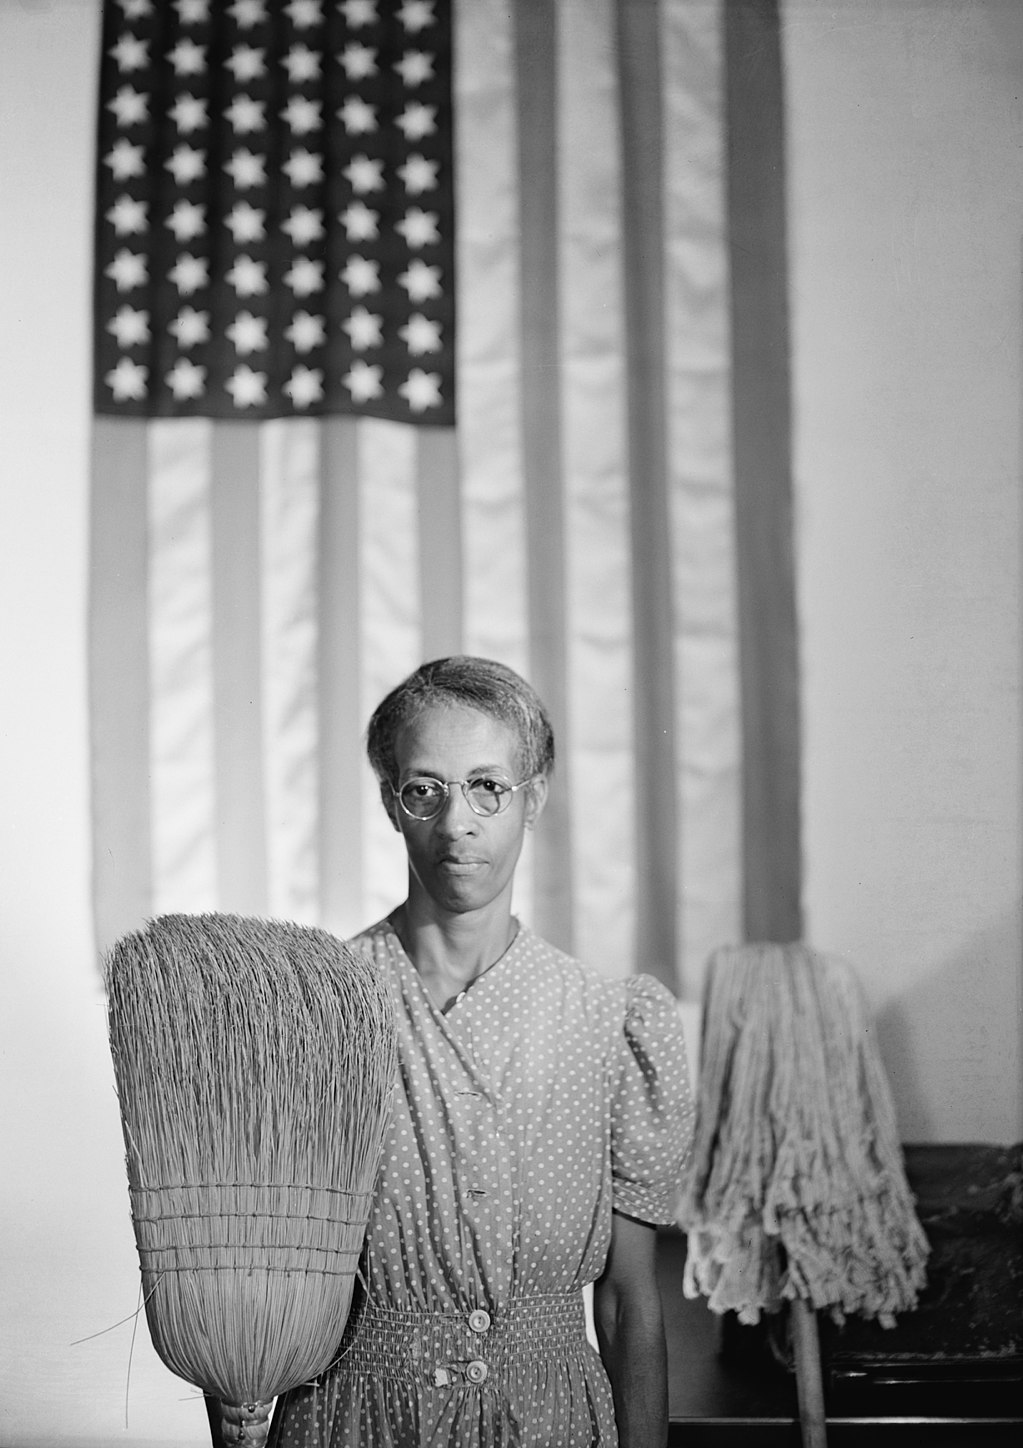
\includegraphics[width=0.95\textwidth]{img/1024px-Gordon_Parks_-_American_Gothic.jpg}
% \end{center}
%
% \end{frame}
%
% %%%%%%%%%%%%%%%%%%%%%%%%%%%%%%%%%%%%%%%%%%%%%%%%%%%
% \begin{frame}{FSA-OWI: Dorothea Lange}
%
% \begin{center}
% 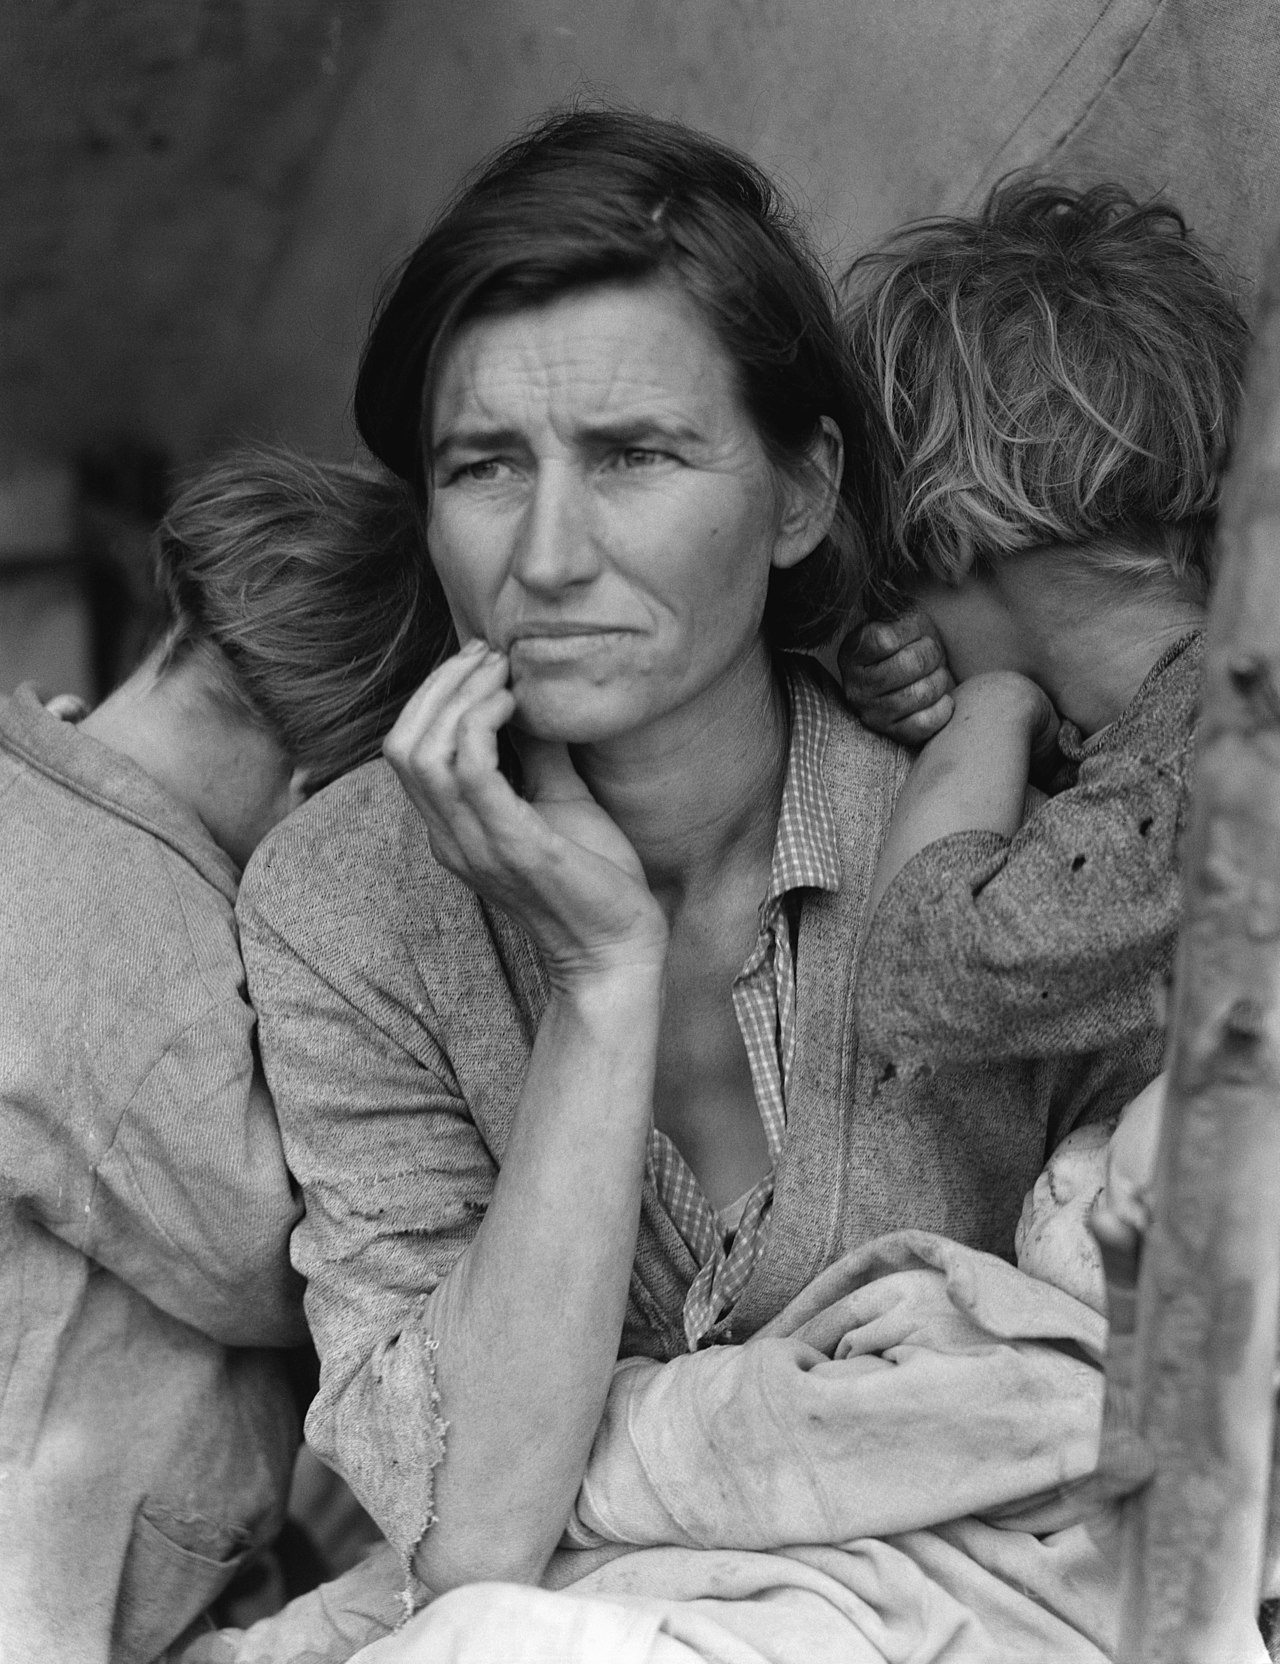
\includegraphics[width=0.95\textwidth]{img/1280px-Lange-MigrantMother02.jpg}
% \end{center}
%
% \end{frame}
%
% %%%%%%%%%%%%%%%%%%%%%%%%%%%%%%%%%%%%%%%%%%%%%%%%%%%
% \begin{frame}{FSA-OWI: Arthur Rothstein}
%
% \begin{center}
% \includegraphics[width=0.95\textwidth]{img/Farmer_walking_in_dust_storm_Cimarron_County_Oklahoma2.jpg}
% \end{center}
%
% \end{frame}
%
% %%%%%%%%%%%%%%%%%%%%%%%%%%%%%%%%%%%%%%%%%%%%%%%%%%%
% \begin{frame}{FSA-OWI: Walker Evans}
%
% \begin{center}
% 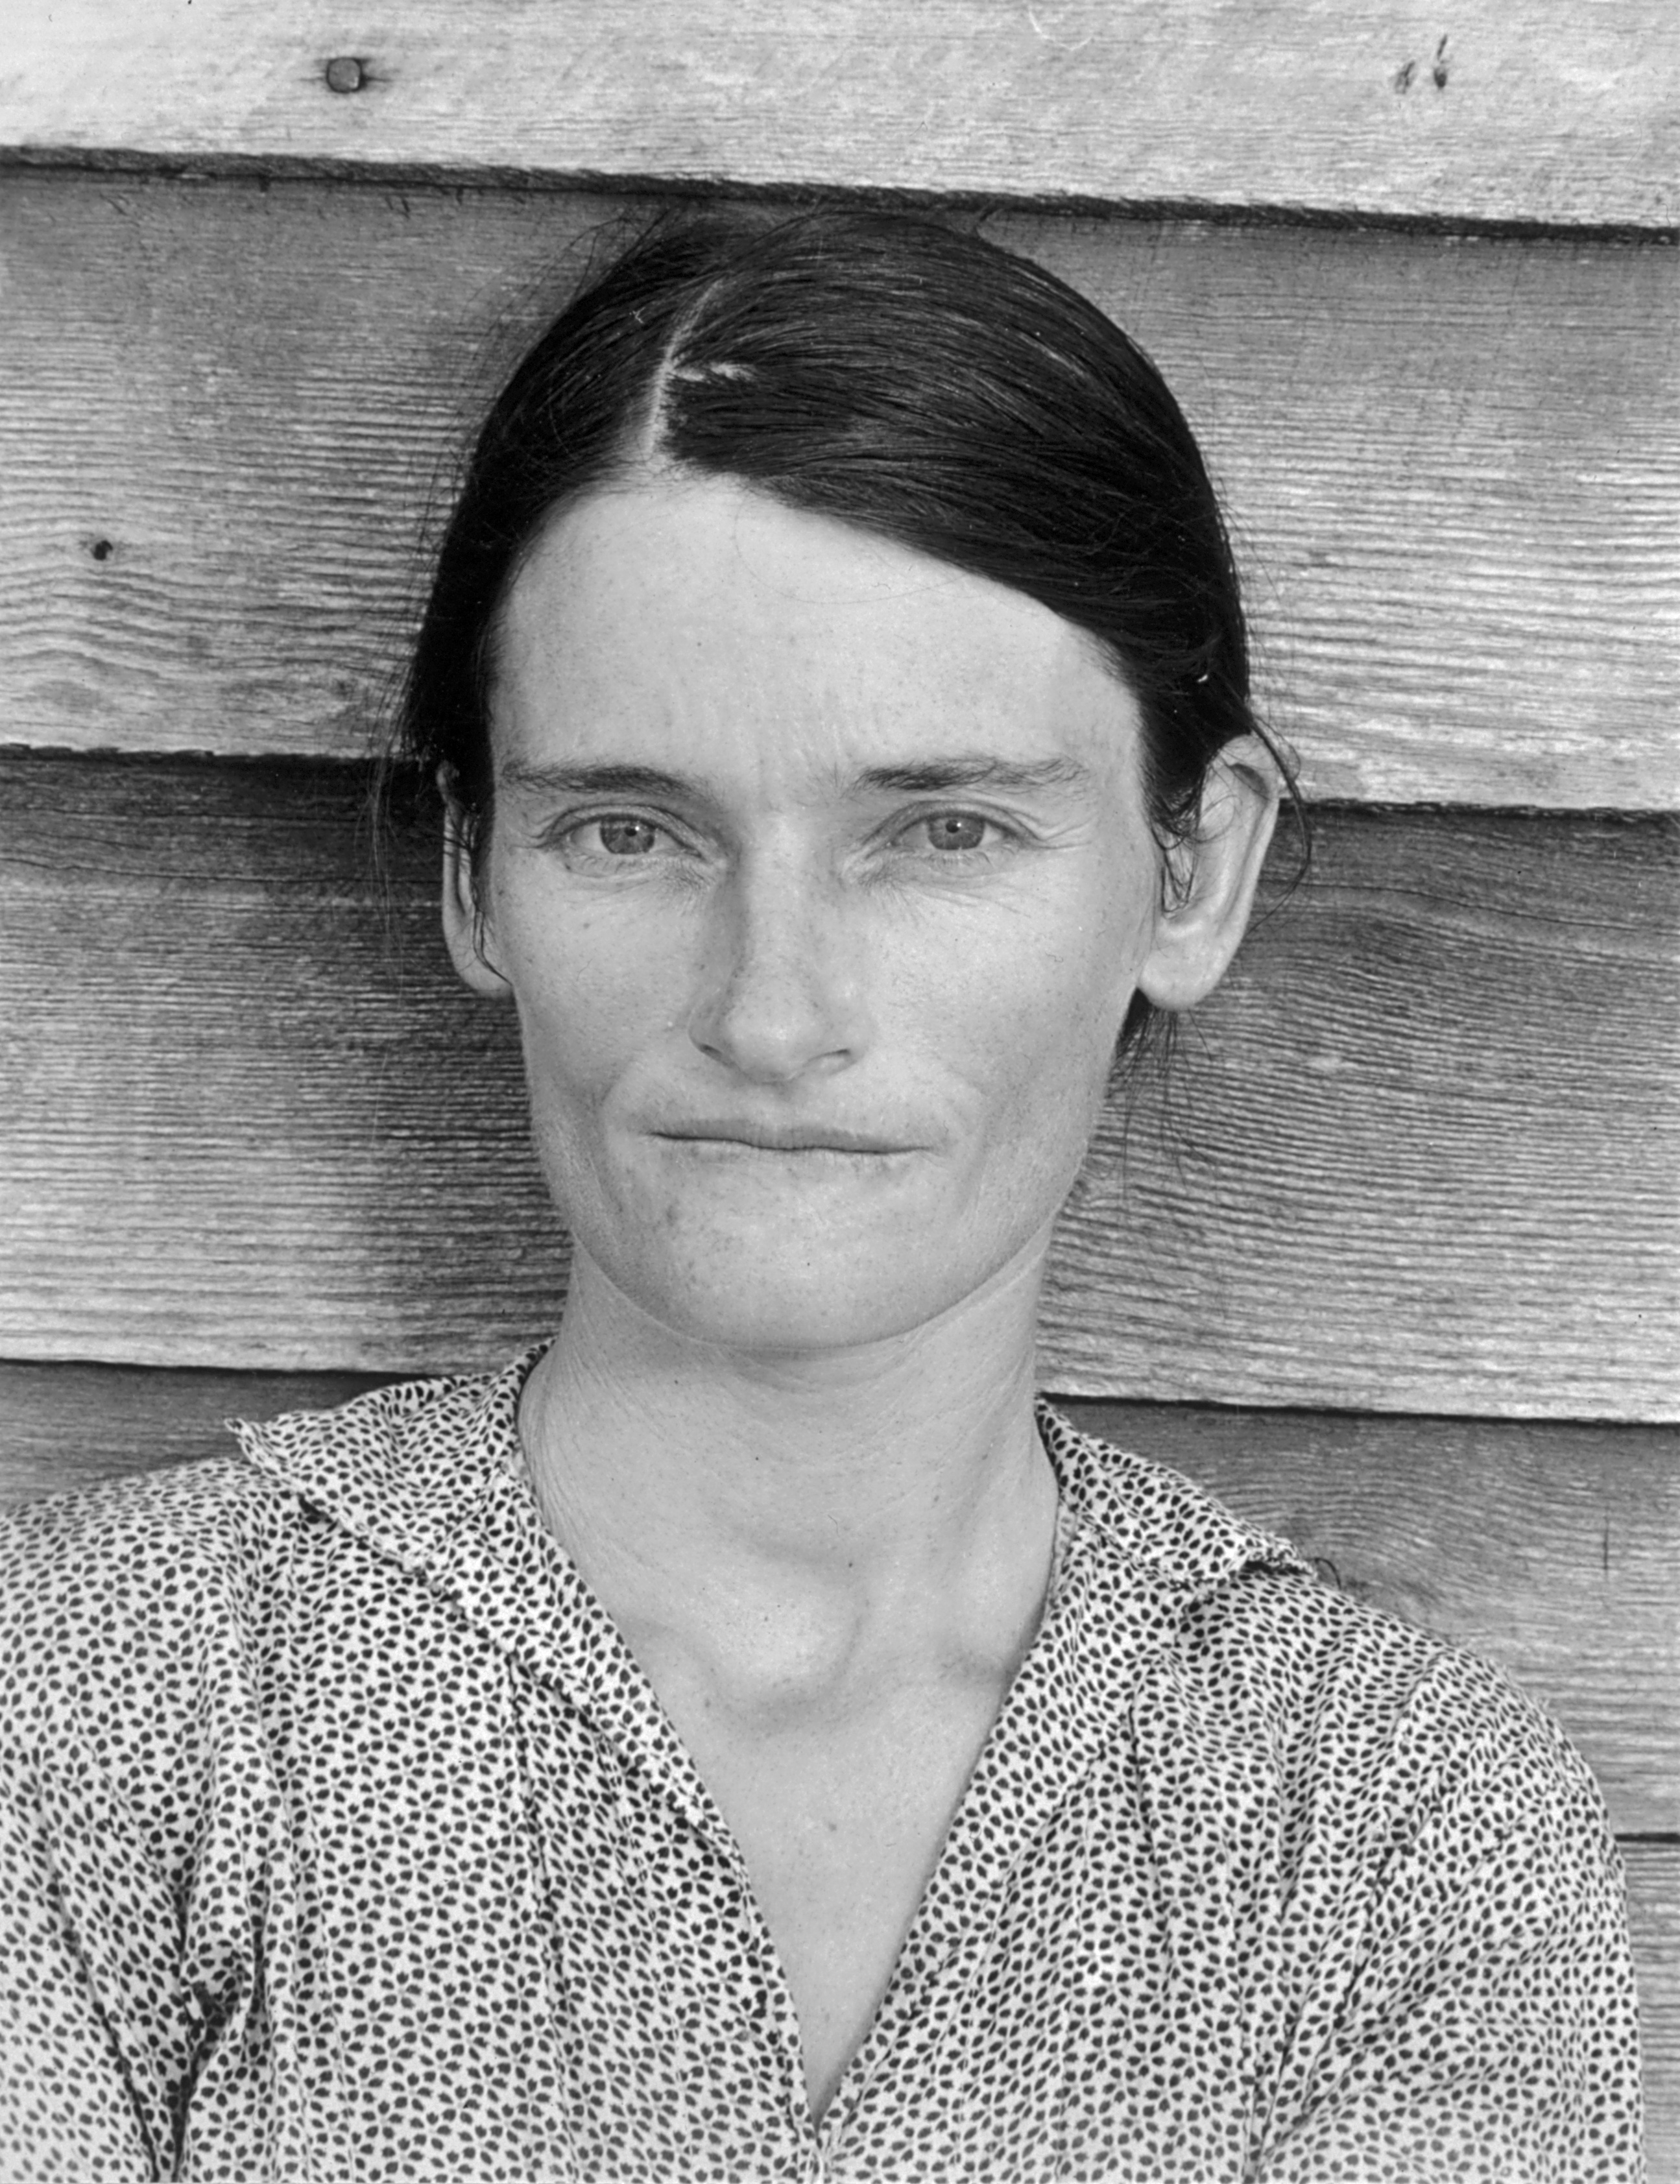
\includegraphics[height=0.8\textheight]{img/Allie_Mae_Burroughs_print.jpg}
% \end{center}
%
% \end{frame}

%%%%%%%%%%%%%%%%%%%%%%%%%%%%%%%%%%%%%%%%%%%%%%%%%%%
\begin{frame}{FSA-OWI}

Apply to 1610 color photographs from the Farm Security Administration-Office of War
Information Collection (FSA-OWI):

\begin{itemize}
\item it is a part of one of the most famous and researched photography archives from the United States  \pause
\item held by a library that is invested in open access and
encourages experimentation with their digital collections  \pause
\item indicative of many documentary photography collections held in GLAM
institutions  \pause
\item a collection we have worked with through out Photogrammar project since 2010
\end{itemize}

\end{frame}

%%%%%%%%%%%%%%%%%%%%%%%%%%%%%%%%%%%%%%%%%%%%%%%%%%%
\begin{frame}{Photogrammar}

\begin{center}
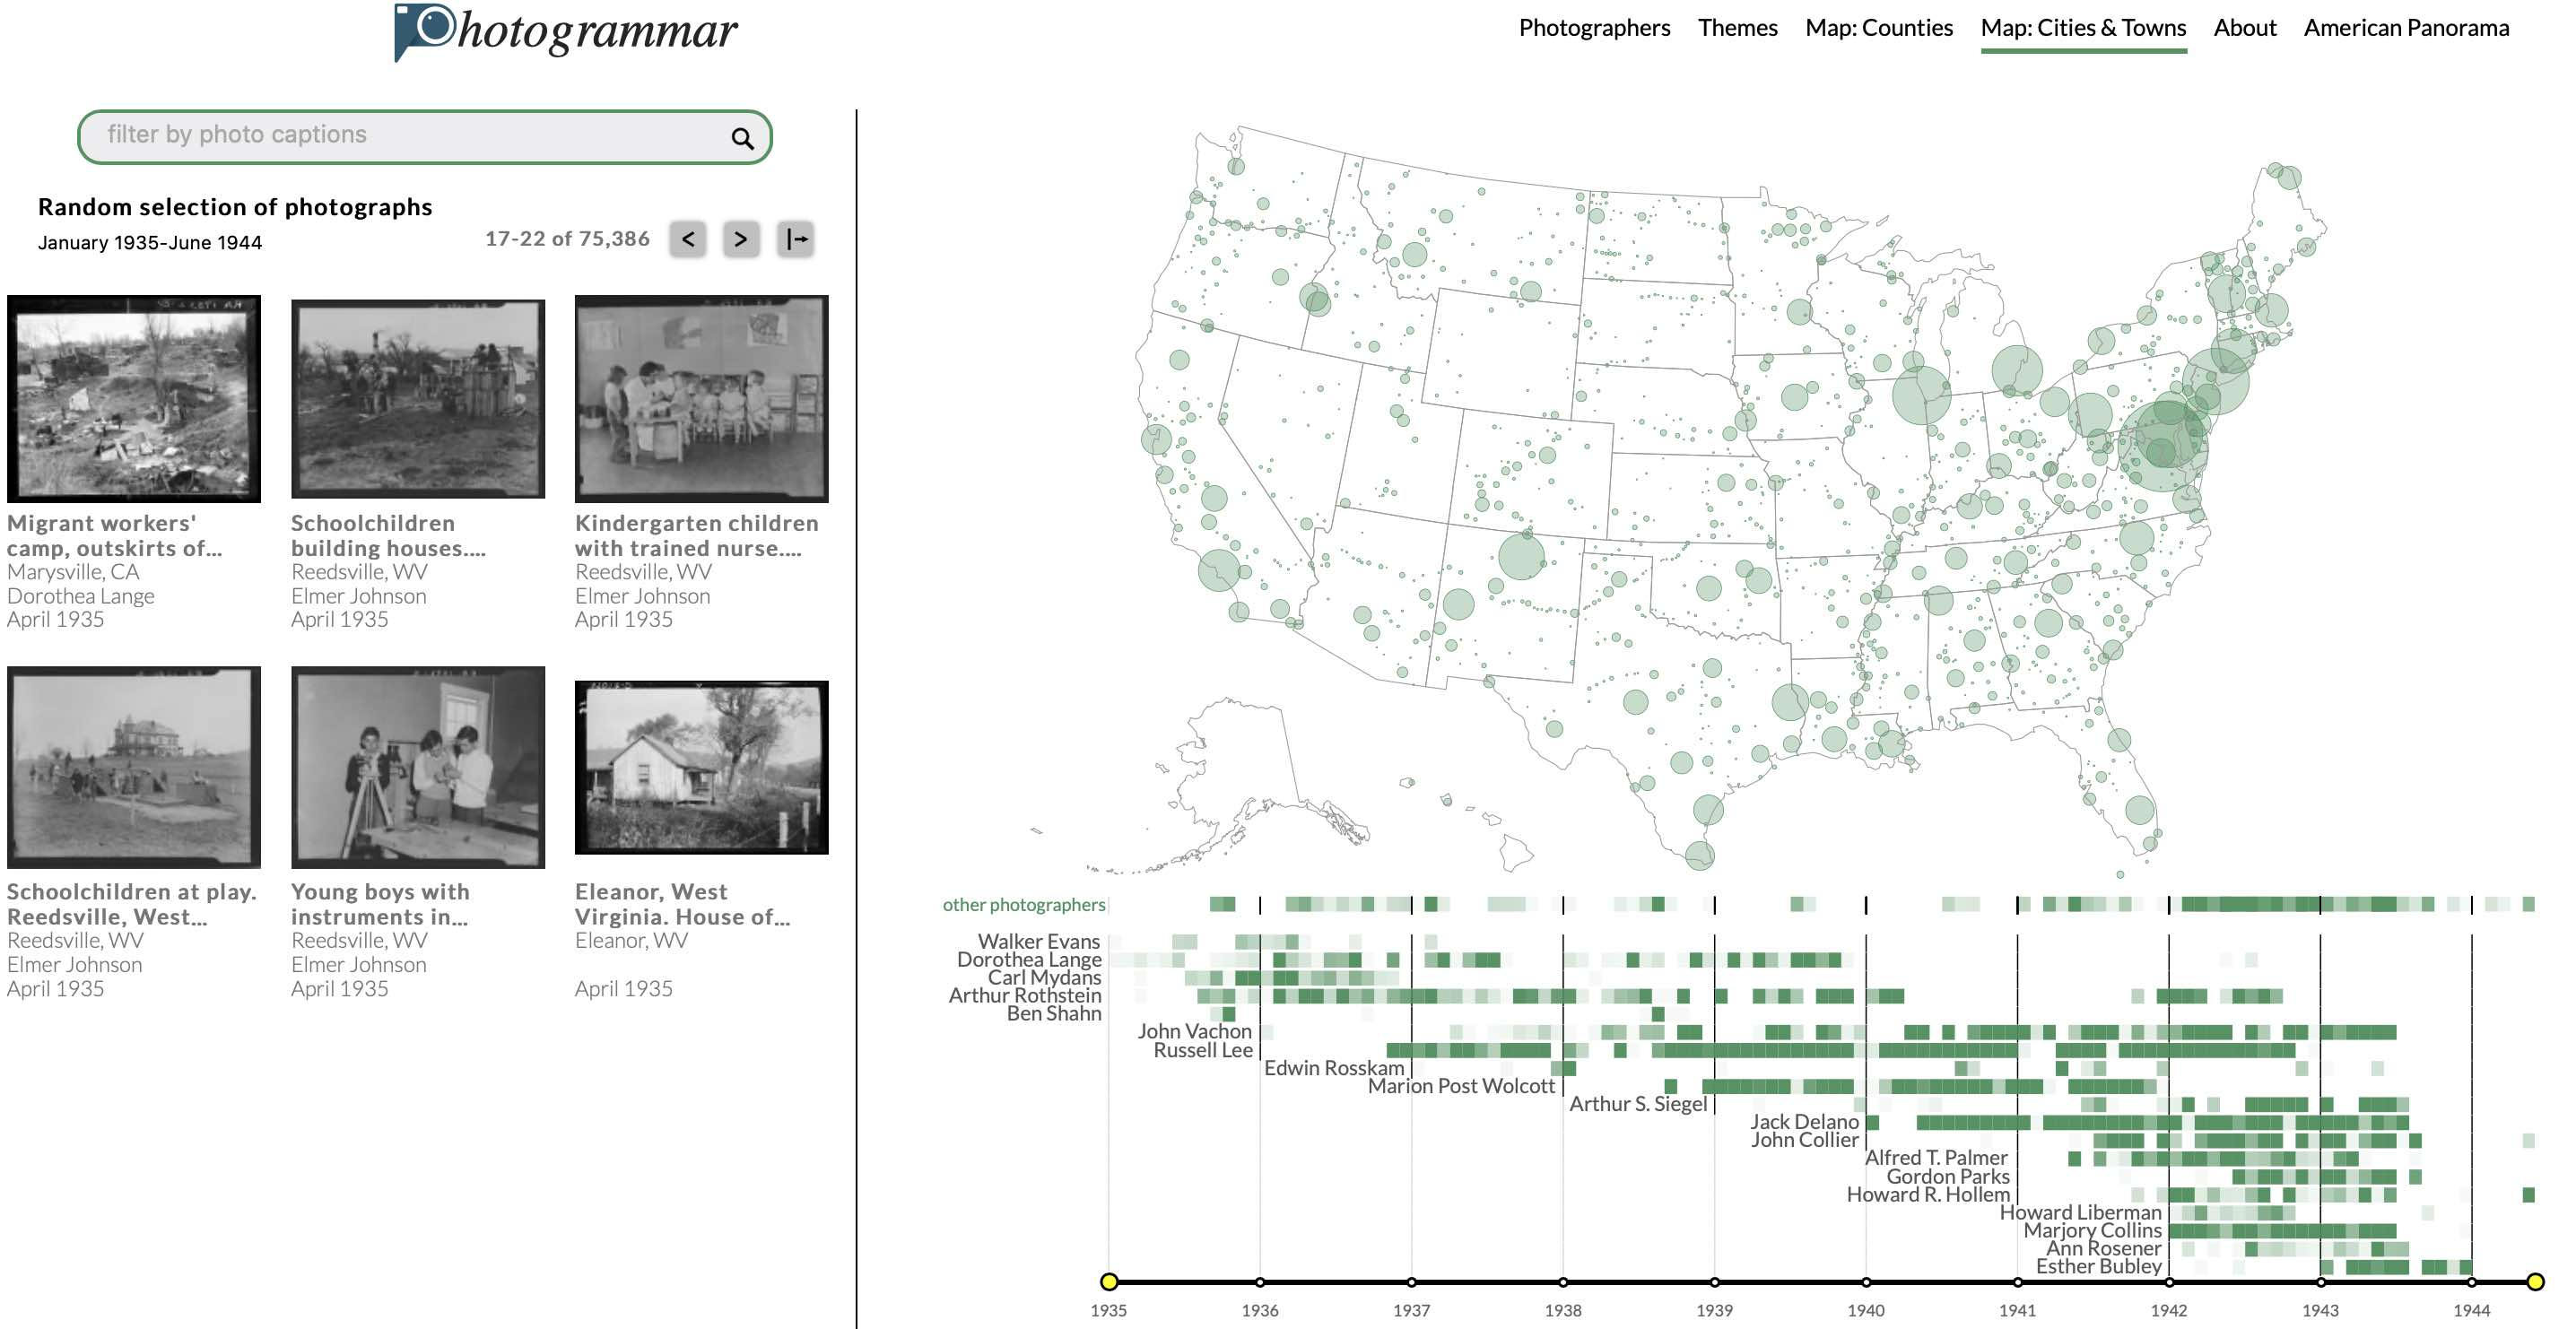
\includegraphics[height=0.8\textheight]{img/pgram1.jpg}
\end{center}

\end{frame}
%
% %%%%%%%%%%%%%%%%%%%%%%%%%%%%%%%%%%%%%%%%%%%%%%%%%%%
% \begin{frame}{Photogrammar}
%
% \begin{center}
% 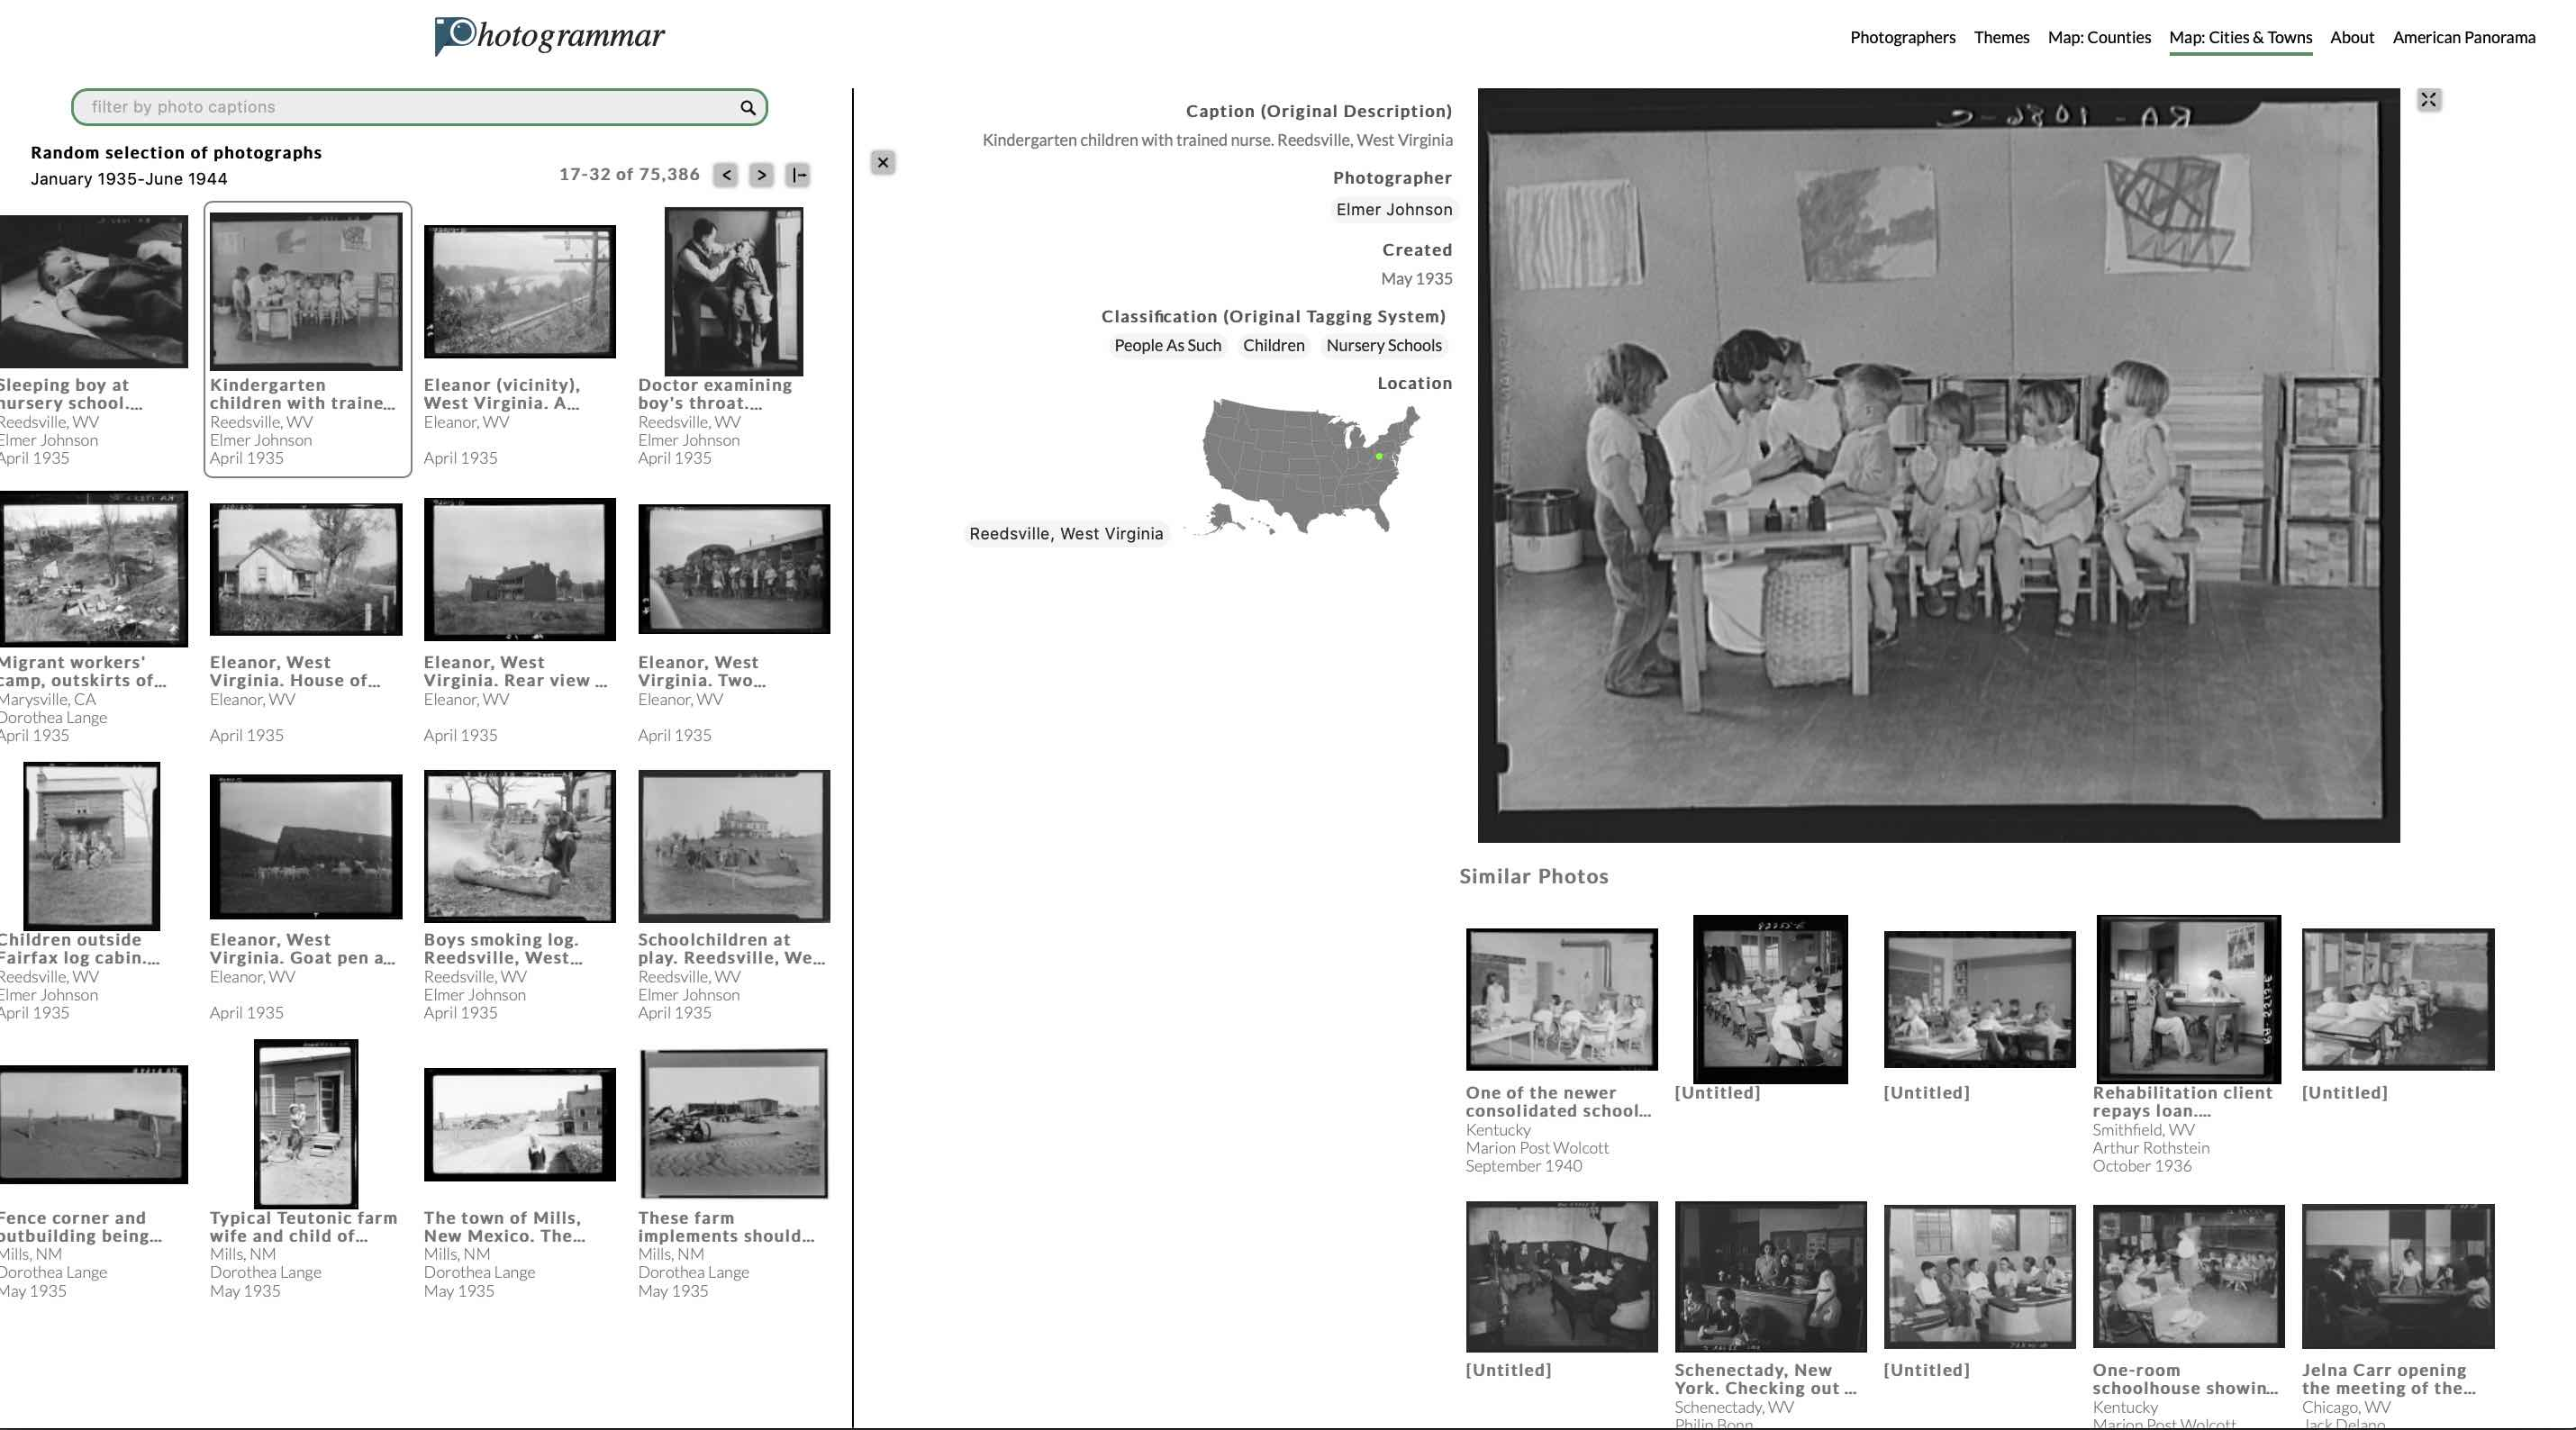
\includegraphics[height=0.8\textheight]{img/pgram2.jpg}
% \end{center}
%
% \end{frame}

%%%%%%%%%%%%%%%%%%%%%%%%%%%%%%%%%%%%%%%%%%%%%%%%%%%
\section{Previous Approaches}

%%%%%%%%%%%%%%%%%%%%%%%%%%%%%%%%%%%%%%%%%%%%%%%%%%%
\begin{frame}{}

Computer vision methods for creating structured data from still photography:

\begin{itemize}
\item object detection
\item automatic free-form captions
\item image embeddings
\end{itemize}

\end{frame}

%%%%%%%%%%%%%%%%%%%%%%%%%%%%%%%%%%%%%%%%%%%%%%%%%%%
\begin{frame}{Object Detection}

\orange{Mask R-CNN} instance object classification algorithm (X101-FPN).

Wu, Y., Kirillov, A., Massa, F., Lo, W.-Y., and Girshick, R. (2019). \textit{Detectron2}.

\end{frame}

%%%%%%%%%%%%%%%%%%%%%%%%%%%%%%%%%%%%%%%%%%%%%%%%%%%
\begin{frame}{Object Detection}

\begin{center}
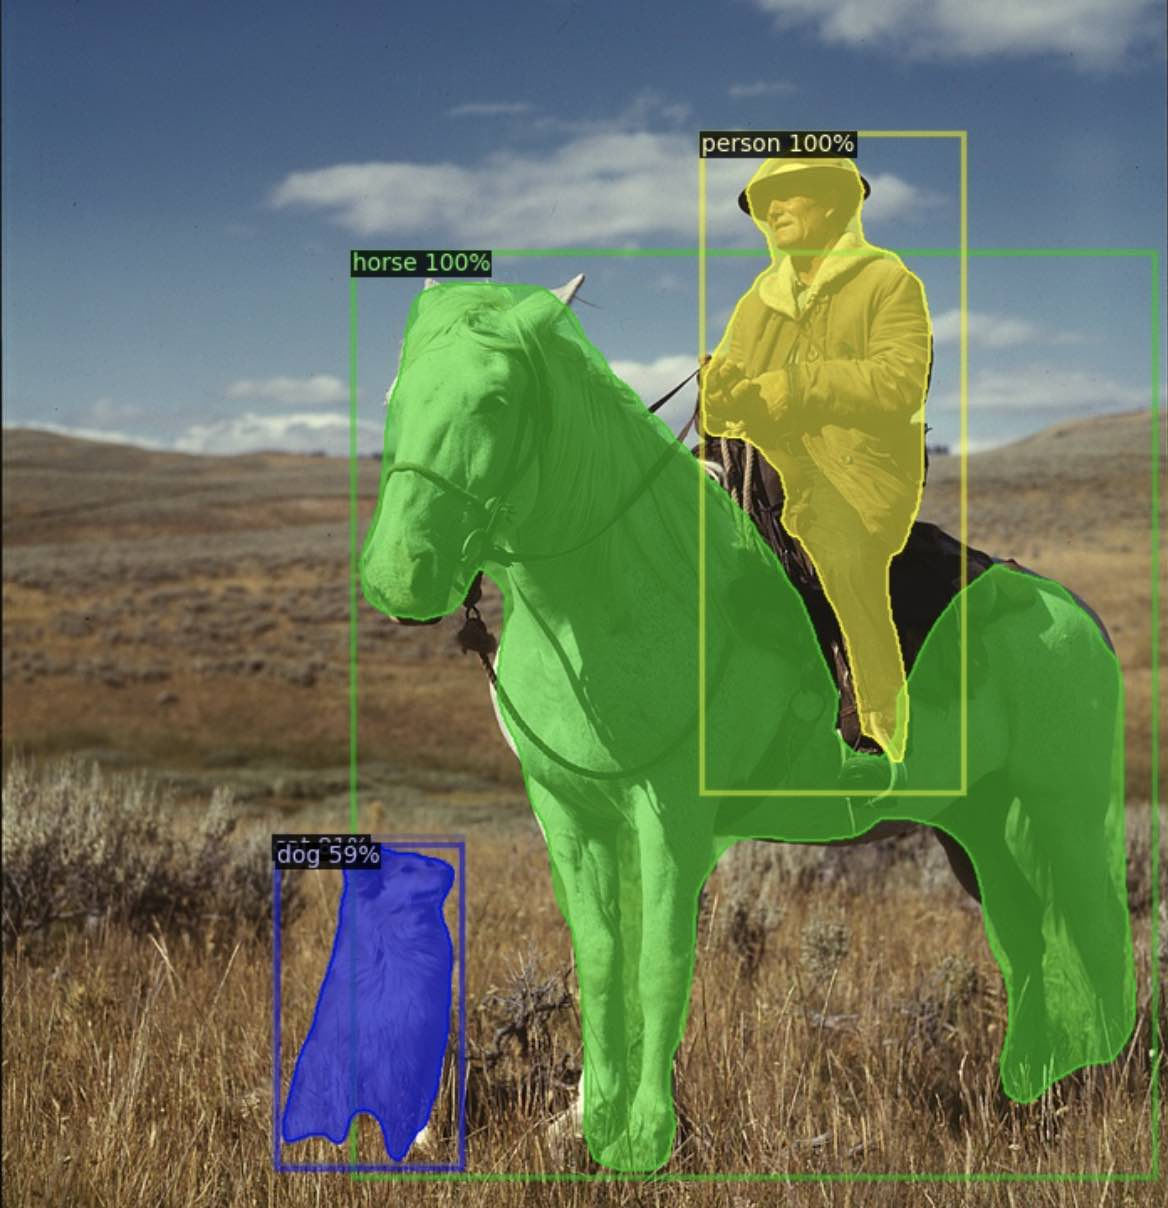
\includegraphics[width=0.95\textwidth]{img/object.jpg}
\end{center}

\end{frame}

%%%%%%%%%%%%%%%%%%%%%%%%%%%%%%%%%%%%%%%%%%%%%%%%%%%
\begin{frame}{Object Detection}

\begin{center}
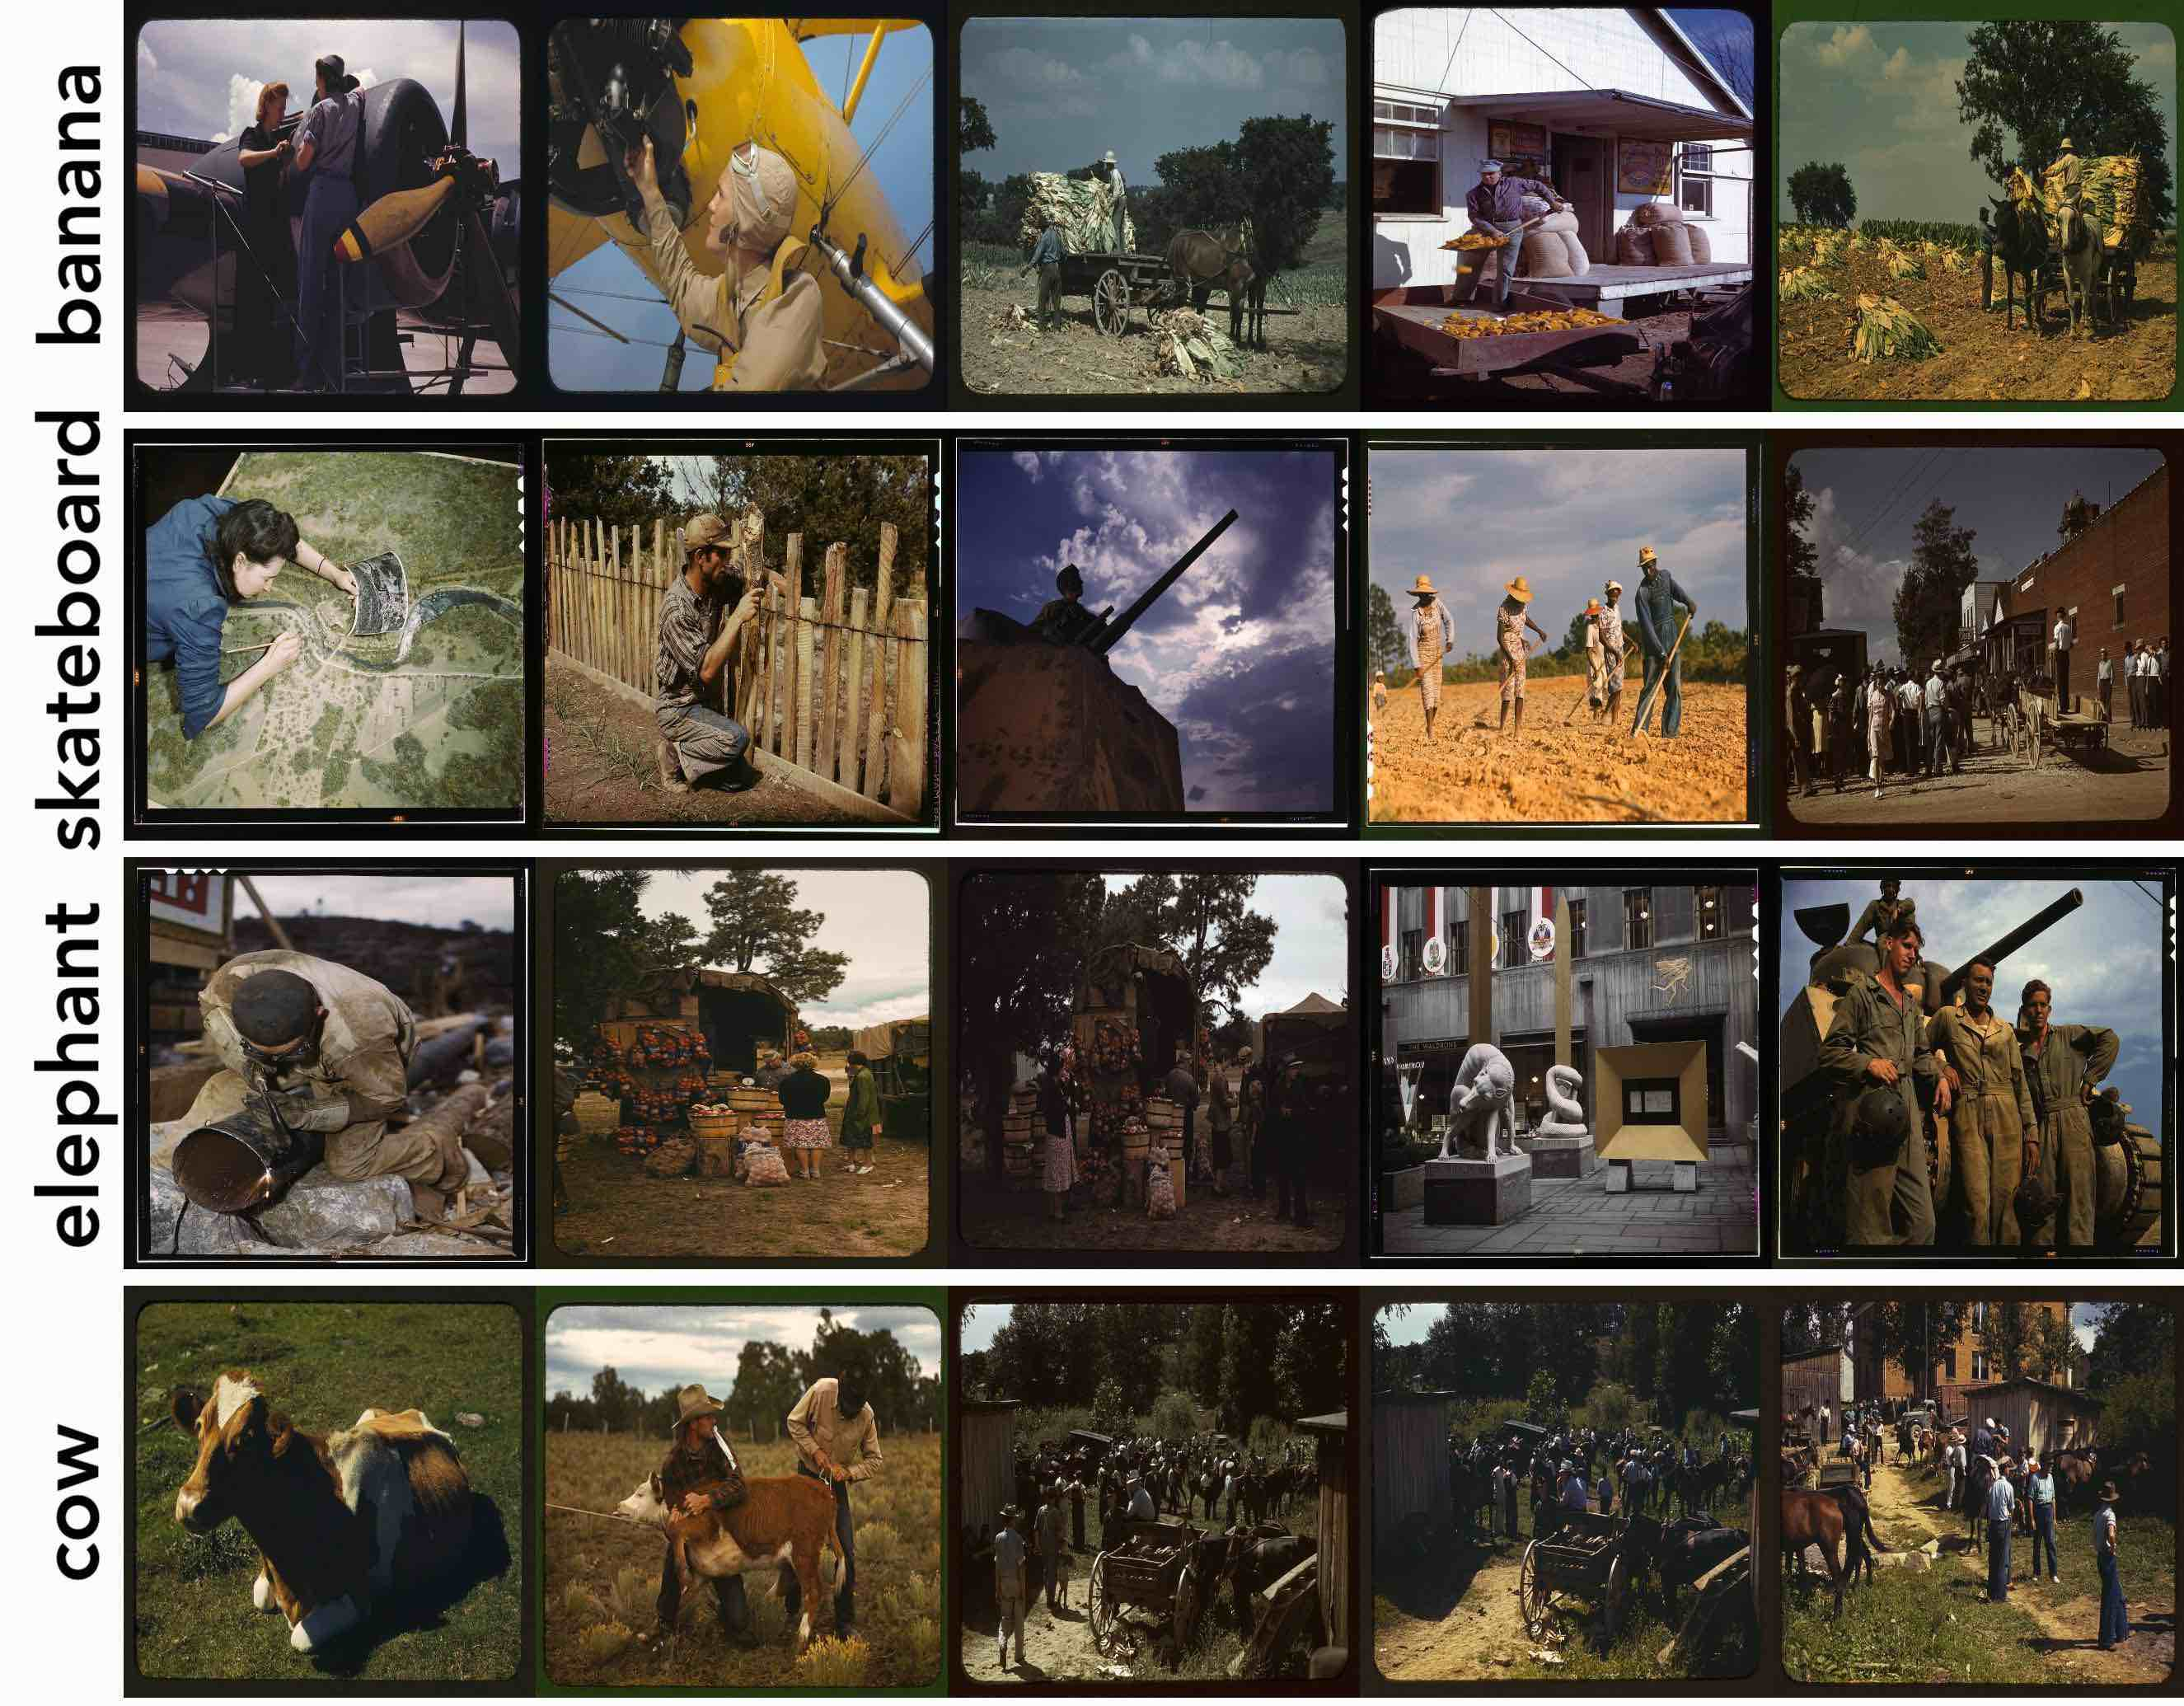
\includegraphics[width=0.95\textwidth]{../figures/max_things_grid_labels_small.jpg}
\end{center}

\end{frame}

%%%%%%%%%%%%%%%%%%%%%%%%%%%%%%%%%%%%%%%%%%%%%%%%%%%
\begin{frame}{Object Detection}

\begin{center}
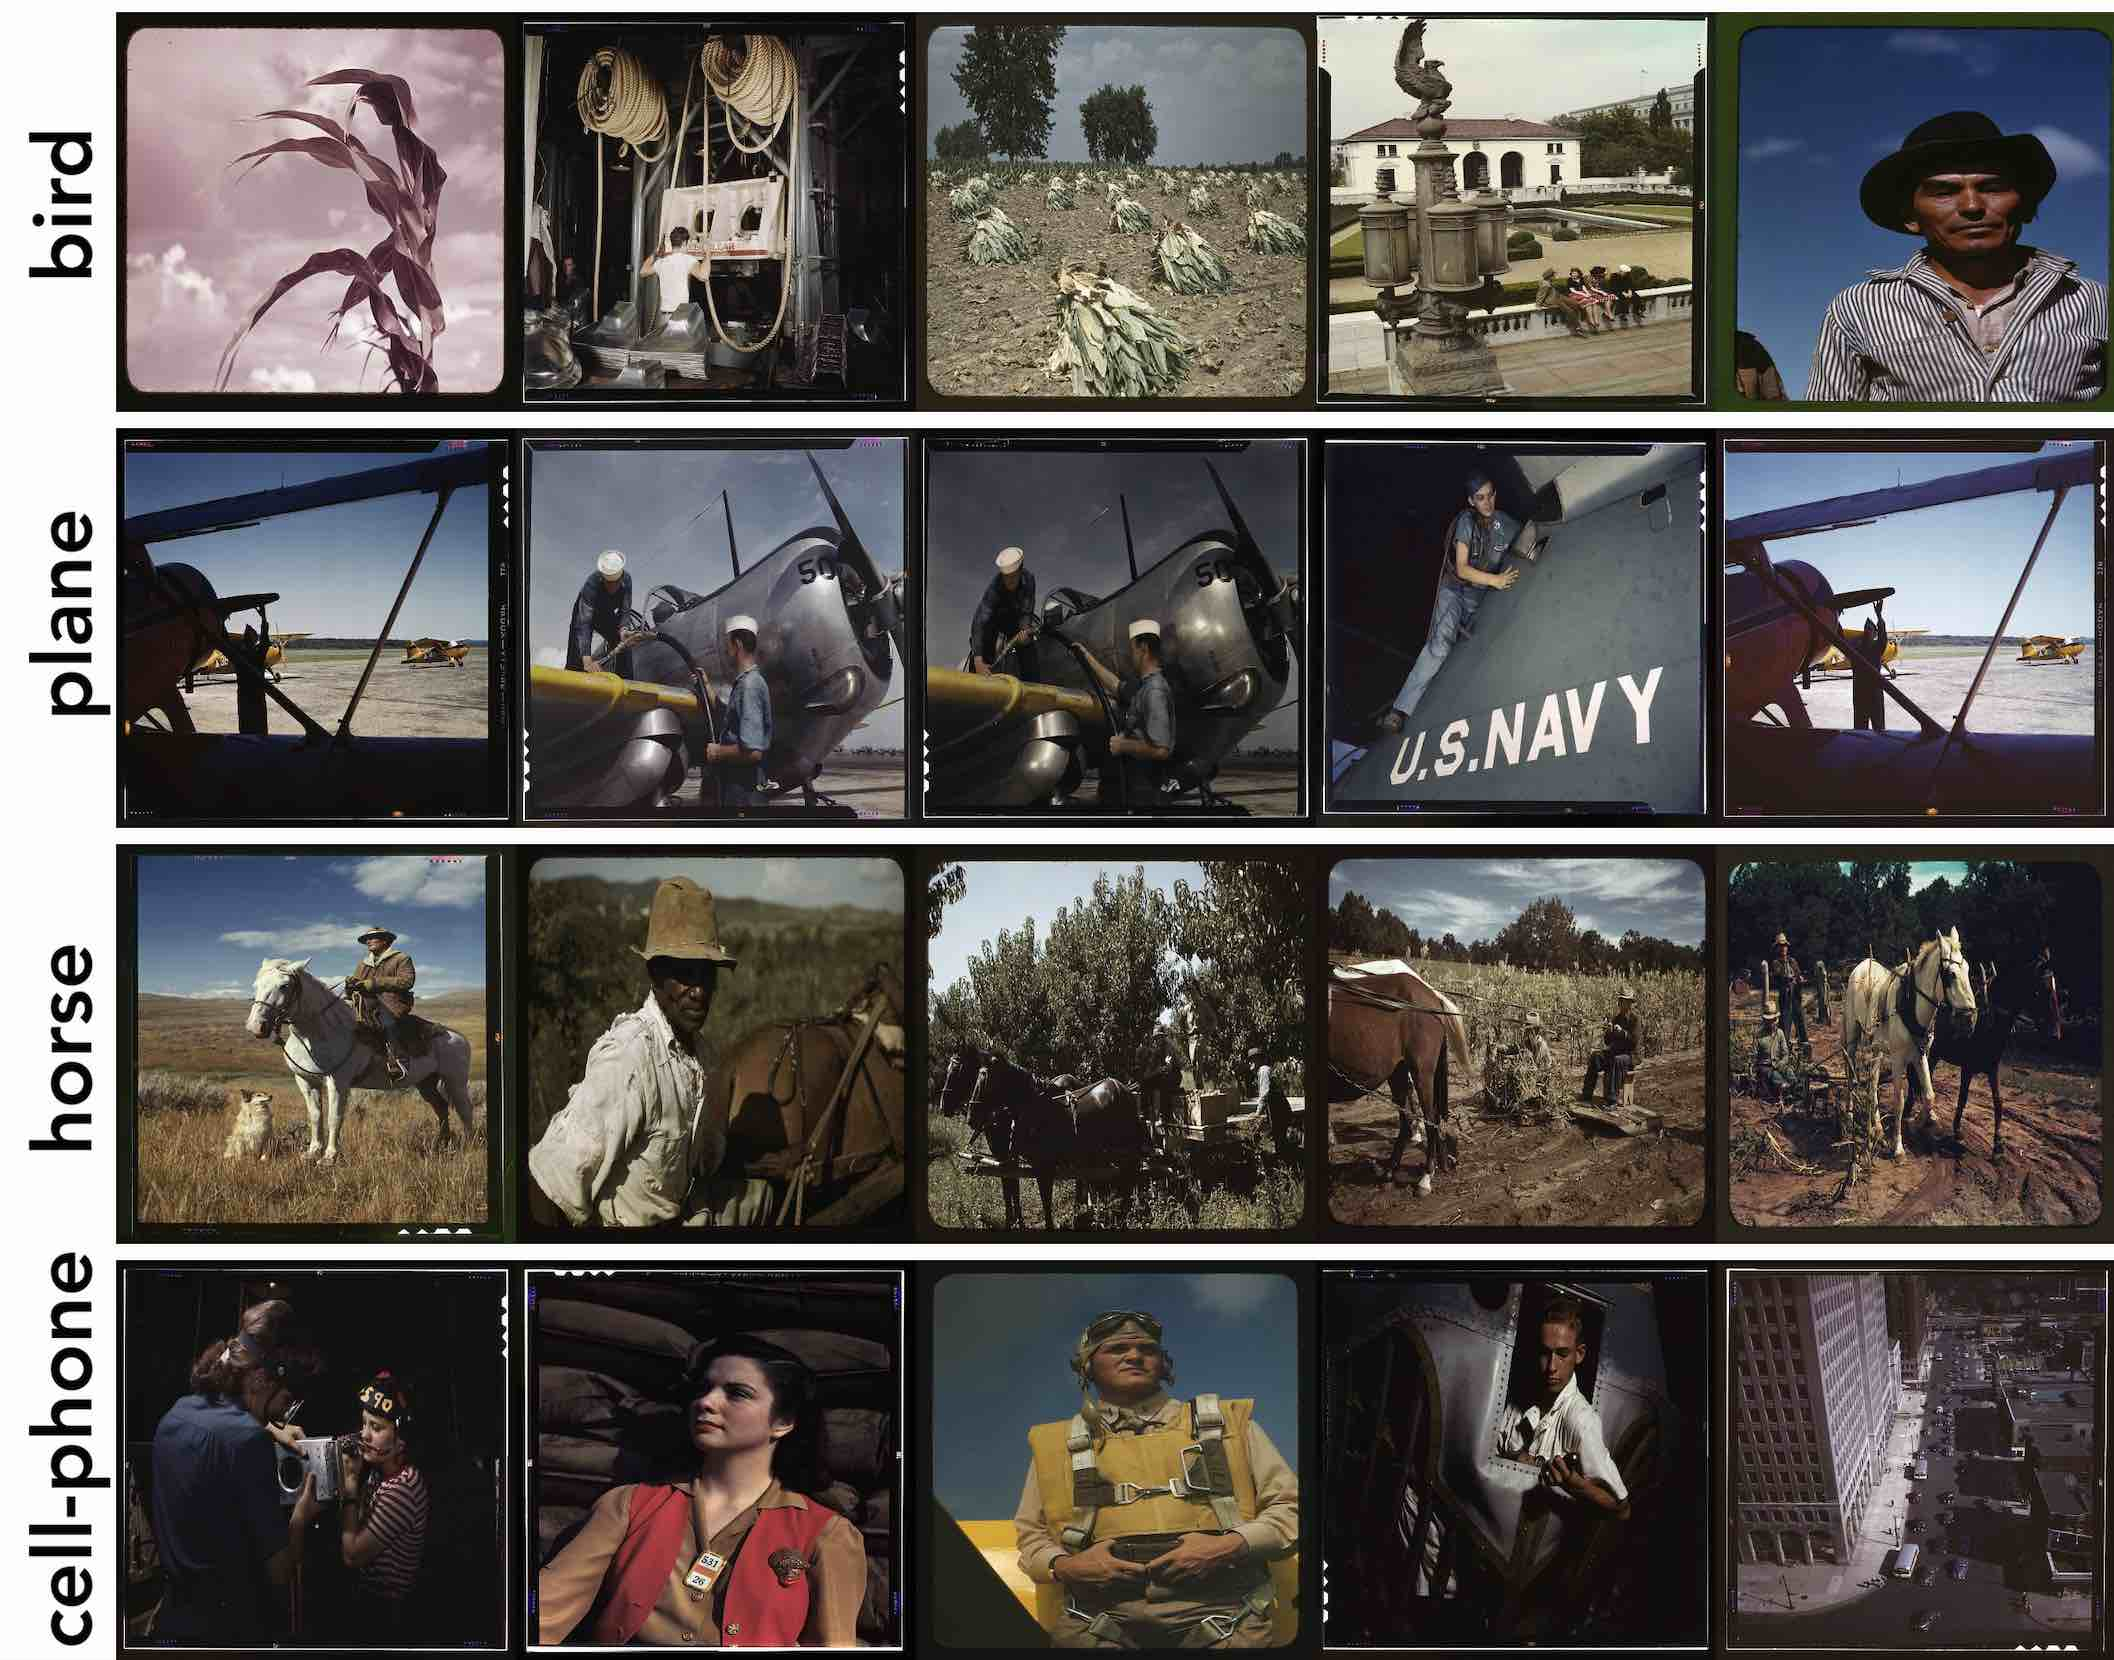
\includegraphics[width=0.95\textwidth]{../figures/max_things_grid_labels_small_bottom.jpg}
\end{center}

\end{frame}

%%%%%%%%%%%%%%%%%%%%%%%%%%%%%%%%%%%%%%%%%%%%%%%%%%%
\begin{frame}{Automatic Captions}

\orange{Show, attend and tell}

Xu, Kelvin, et al. ``Show, attend and tell: Neural image caption generation with visual
attention.'' \textit{International conference on machine learning}. 2015.

\end{frame}

%%%%%%%%%%%%%%%%%%%%%%%%%%%%%%%%%%%%%%%%%%%%%%%%%%%
\begin{frame}{Automatic Captions}

\begin{center}
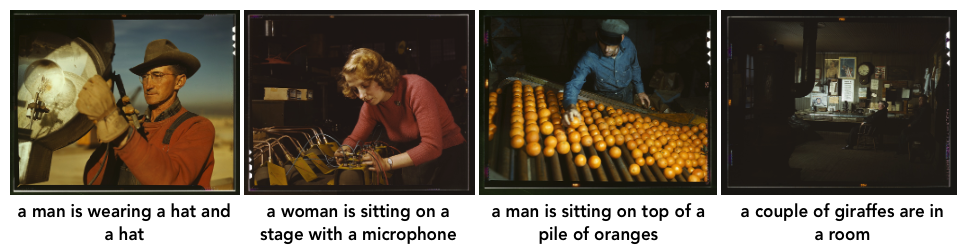
\includegraphics[width=0.95\textwidth]{../figures/captions.png}
\end{center}

\end{frame}

%%%%%%%%%%%%%%%%%%%%%%%%%%%%%%%%%%%%%%%%%%%%%%%%%%%
\begin{frame}{Image Embedding}

\orange{VGG-19}

K. Simonyan, A. Zisserman ``Very Deep Convolutional Networks for Large-Scale Image
Recognition.'' \textit{arXiv:1409.1556}

\end{frame}

%%%%%%%%%%%%%%%%%%%%%%%%%%%%%%%%%%%%%%%%%%%%%%%%%%%
\begin{frame}{Image Embeddings}

\begin{center}
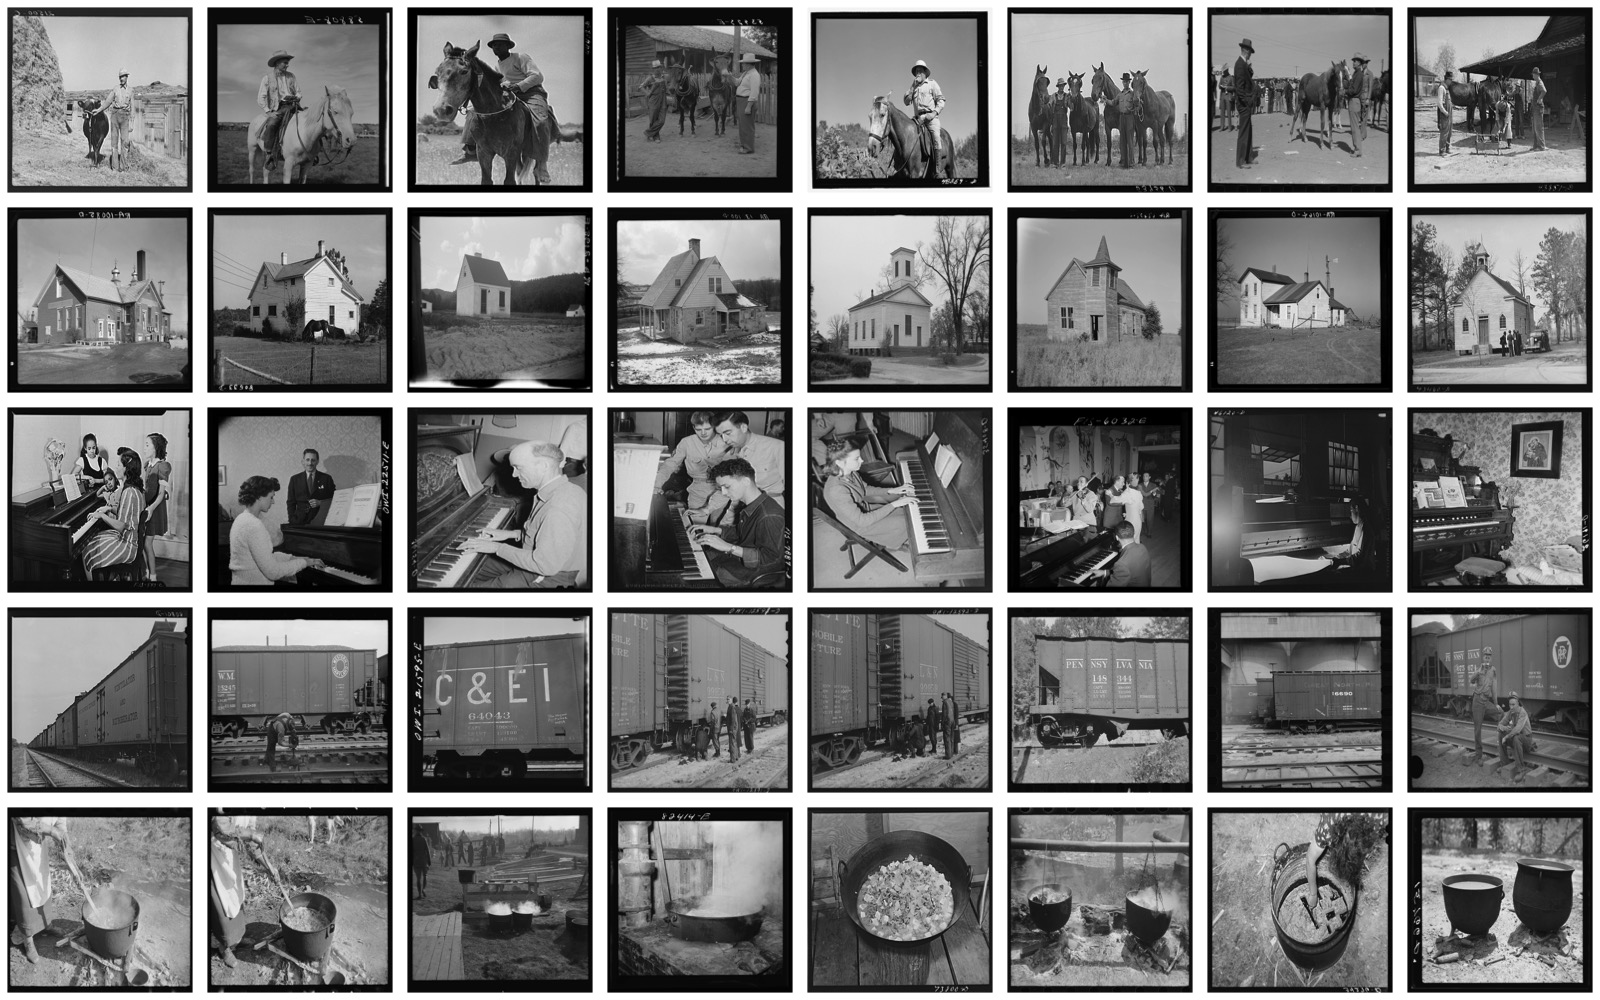
\includegraphics[width=0.95\textwidth]{img/fig3.jpg}
\end{center}

\end{frame}

%%%%%%%%%%%%%%%%%%%%%%%%%%%%%%%%%%%%%%%%%%%%%%%%%%%
\section{Image Segmentation}

%%%%%%%%%%%%%%%%%%%%%%%%%%%%%%%%%%%%%%%%%%%%%%%%%%%
\begin{frame}{Image Embedding}

\orange{COCO-stuff}

Caesar, H., Uijlings, J., \& Ferrari, V. (2018). ``COCO-stuff: Thing and stuff classes
in context.'' In: \textit{Proceedings of the IEEE Conference on Computer Vision and Pattern
Recognition} (pp. 1209-1218).

\end{frame}


%%%%%%%%%%%%%%%%%%%%%%%%%%%%%%%%%%%%%%%%%%%%%%%%%%%
\begin{frame}{}
  \fontsize{9}{11}\selectfont
  \centering

  \begin{tabular}{lll}
   \hline
  \textbf{Group} & \textbf{Meta} & \textbf{Categories} \\
   \hline
   indoor & ceiling & ceiling-tile \\
   indoor & floor & floor-wood; floor-stone; floor-tile; floor-marble; carpet \\
   indoor & food & fruit; vegetable; salad \\
   indoor & furniture & cabinet; cupboard; counter; desk; door; light; mirror; shelf; stairs; table \\
   indoor & rawmaterial & cardboard; metal; paper; plastic \\
   indoor & textile & banner; blanket; curtain; cloth; clothes; napkin; mat; pillow; rug; towel \\
   indoor & wall & wall-brick; wall-stone; wall-tile; wall-wood; wall-panel; wall-concrete \\
   indoor & window & window-blind \\ \hline
   outdoor & building & bridge; house; roof; skyscraper; tent \\
   outdoor & ground & dirt; gravel; pavement; platform; playingfield; railroad; road; sand; snow; mud \\
   outdoor & plant & flower; grass; tree; bush; leaves; branch; moss; straw \\
   outdoor & sky & clouds \\
   outdoor & solid & mountain; rock; hill; stone; wood \\
   outdoor & structural & fence; net; railing; cage \\
   outdoor & water & river; sea; waterdrops; fog \\
    \hline
  \end{tabular}


\end{frame}

%%%%%%%%%%%%%%%%%%%%%%%%%%%%%%%%%%%%%%%%%%%%%%%%%%%
\begin{frame}{}

\begin{center}
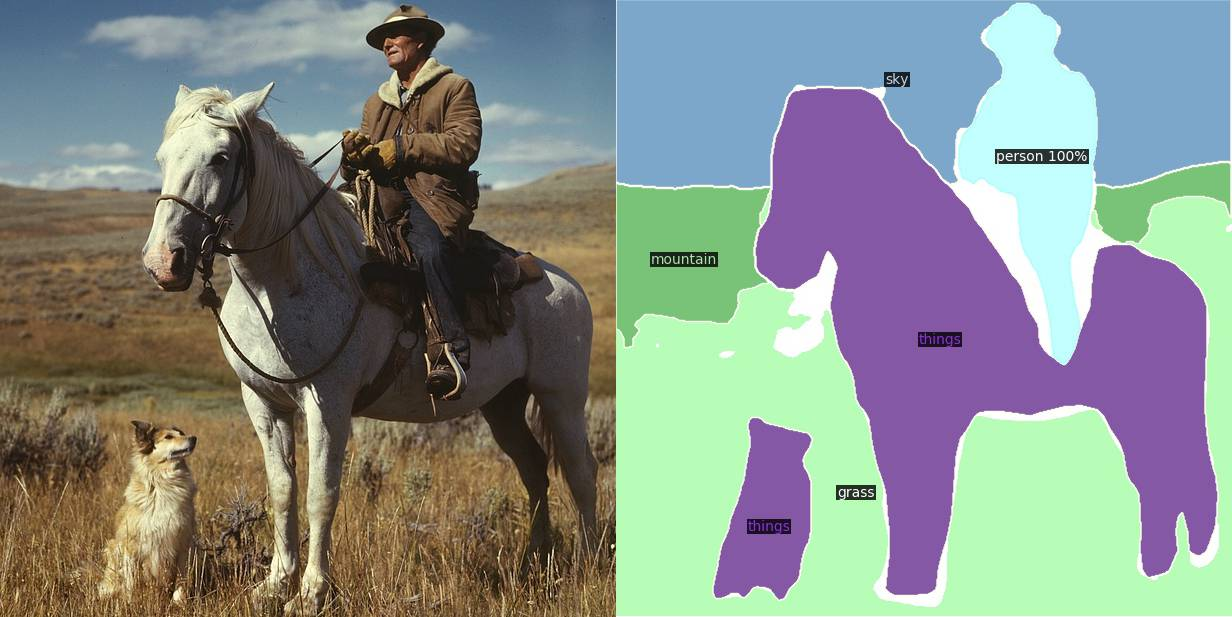
\includegraphics[width=0.95\textwidth]{../figures/segmentation_examples_small.jpg}
\end{center}

\end{frame}

%%%%%%%%%%%%%%%%%%%%%%%%%%%%%%%%%%%%%%%%%%%%%%%%%%%
\begin{frame}{}

\begin{center}
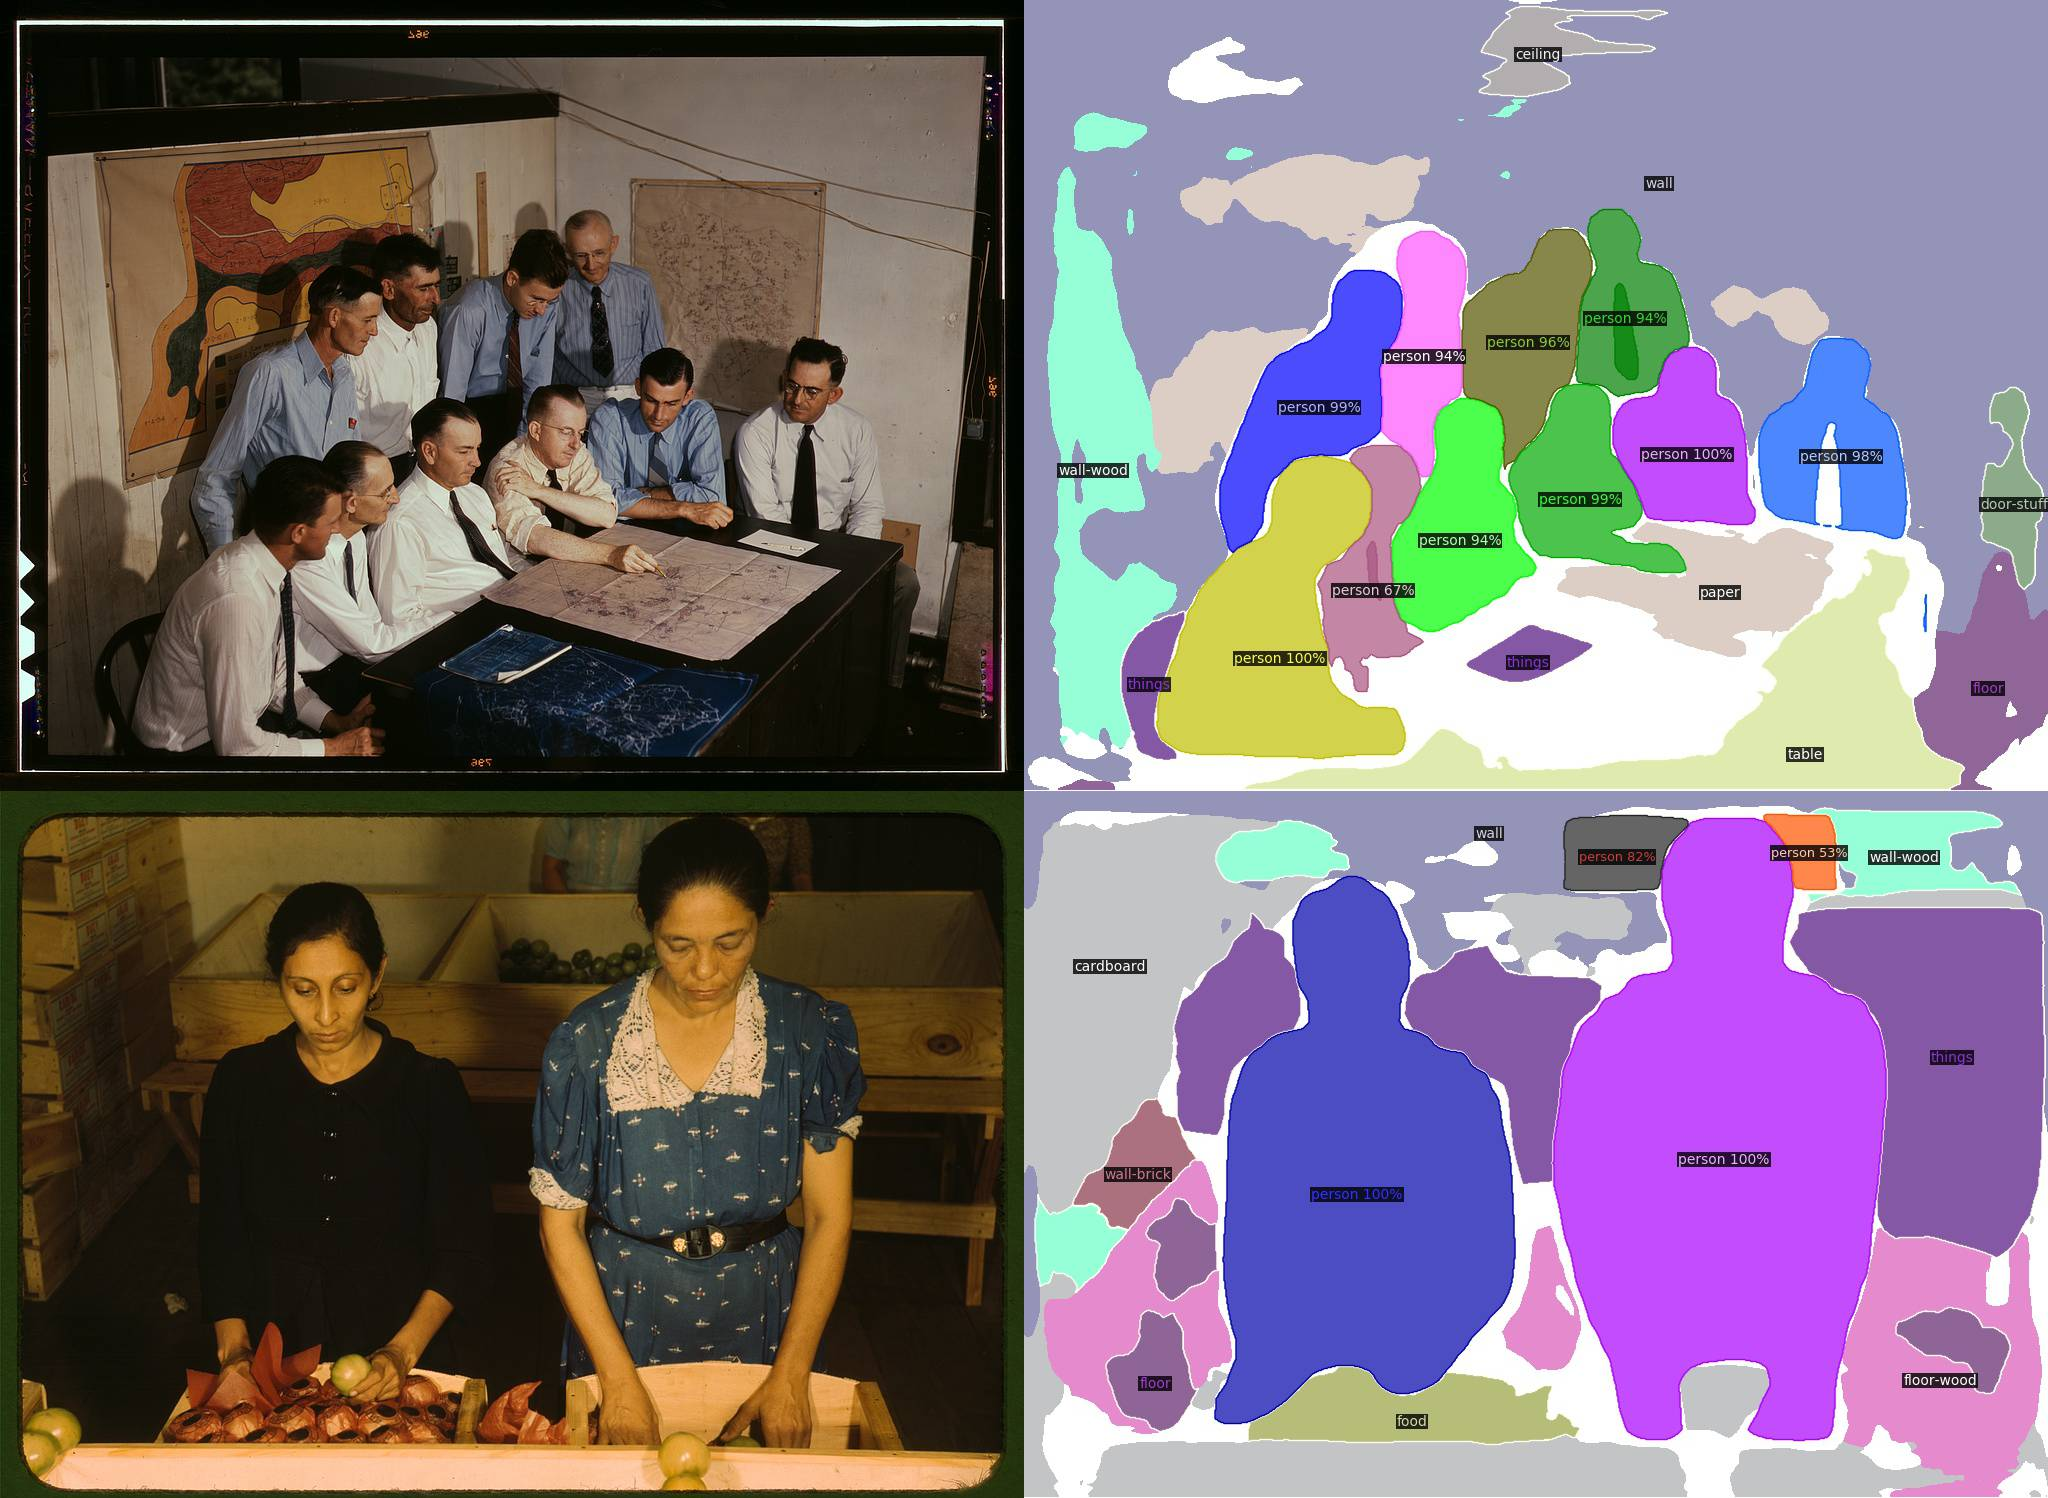
\includegraphics[width=0.95\textwidth]{../figures/segmentation_examples.jpg}
\end{center}

\end{frame}

%%%%%%%%%%%%%%%%%%%%%%%%%%%%%%%%%%%%%%%%%%%%%%%%%%%
\section{Creating Structured Data}

%%%%%%%%%%%%%%%%%%%%%%%%%%%%%%%%%%%%%%%%%%%%%%%%%%%
\begin{frame}{Creating structured data}

Our method:

\begin{itemize}
\item apply the image segementation algorithm
\item record any detected `stuff' region along with the percentage of the image covered
\item record total percentage of `thing' regions
\item record number of `people' regions
\end{itemize}

\end{frame}

%%%%%%%%%%%%%%%%%%%%%%%%%%%%%%%%%%%%%%%%%%%%%%%%%%%
\begin{frame}[fragile]{Web Annotation Data Model: Example I}

\fontsize{9}{11}\selectfont

  \begin{verbatim}
  <http://photogrammar.org/anno1> a oa:Annotation ;
    dcterms:creator <http://photogrammar.org/tarnold2> ;
    dcterms:created "2020-02-19T12:00:00Z" ;
    oa:hasBody [
      a                       pgram:ImageSegmentationRegion ;
      pgram:regionName        <http://example.org/stuff/things> ;
      pgram:regionPercent     32 ;
    ] ;
    oa:hasTarget <http://photogrammar.org/resource/1a35022v> ;
    oa:motivatedBy oa:tagging .
  \end{verbatim}

\end{frame}


%%%%%%%%%%%%%%%%%%%%%%%%%%%%%%%%%%%%%%%%%%%%%%%%%%%
\begin{frame}[fragile]{Web Annotation Data Model: Example II}

\fontsize{9}{11}\selectfont

  \begin{verbatim}
  <http://photogrammar.org/anno2> a oa:Annotation ;
    dcterms:creator <http://photogrammar.org/tarnold2> ;
    dcterms:created "2020-02-19T12:01:00Z" ;
    oa:hasBody [
      a                       pgram:ImageSegmentationRegion ;
      pgram:regionName        <http://example.org/stuff/people> ;
      pgram:regionPercent     6 ;
      pgram:regionCount       1 ;
    ] ;
    oa:hasTarget <http://photogrammar.org/resource/1a35022v> ;
    oa:motivatedBy oa:tagging .
  \end{verbatim}

\end{frame}


%%%%%%%%%%%%%%%%%%%%%%%%%%%%%%%%%%%%%%%%%%%%%%%%%%%
\begin{frame}{}

\begin{center}
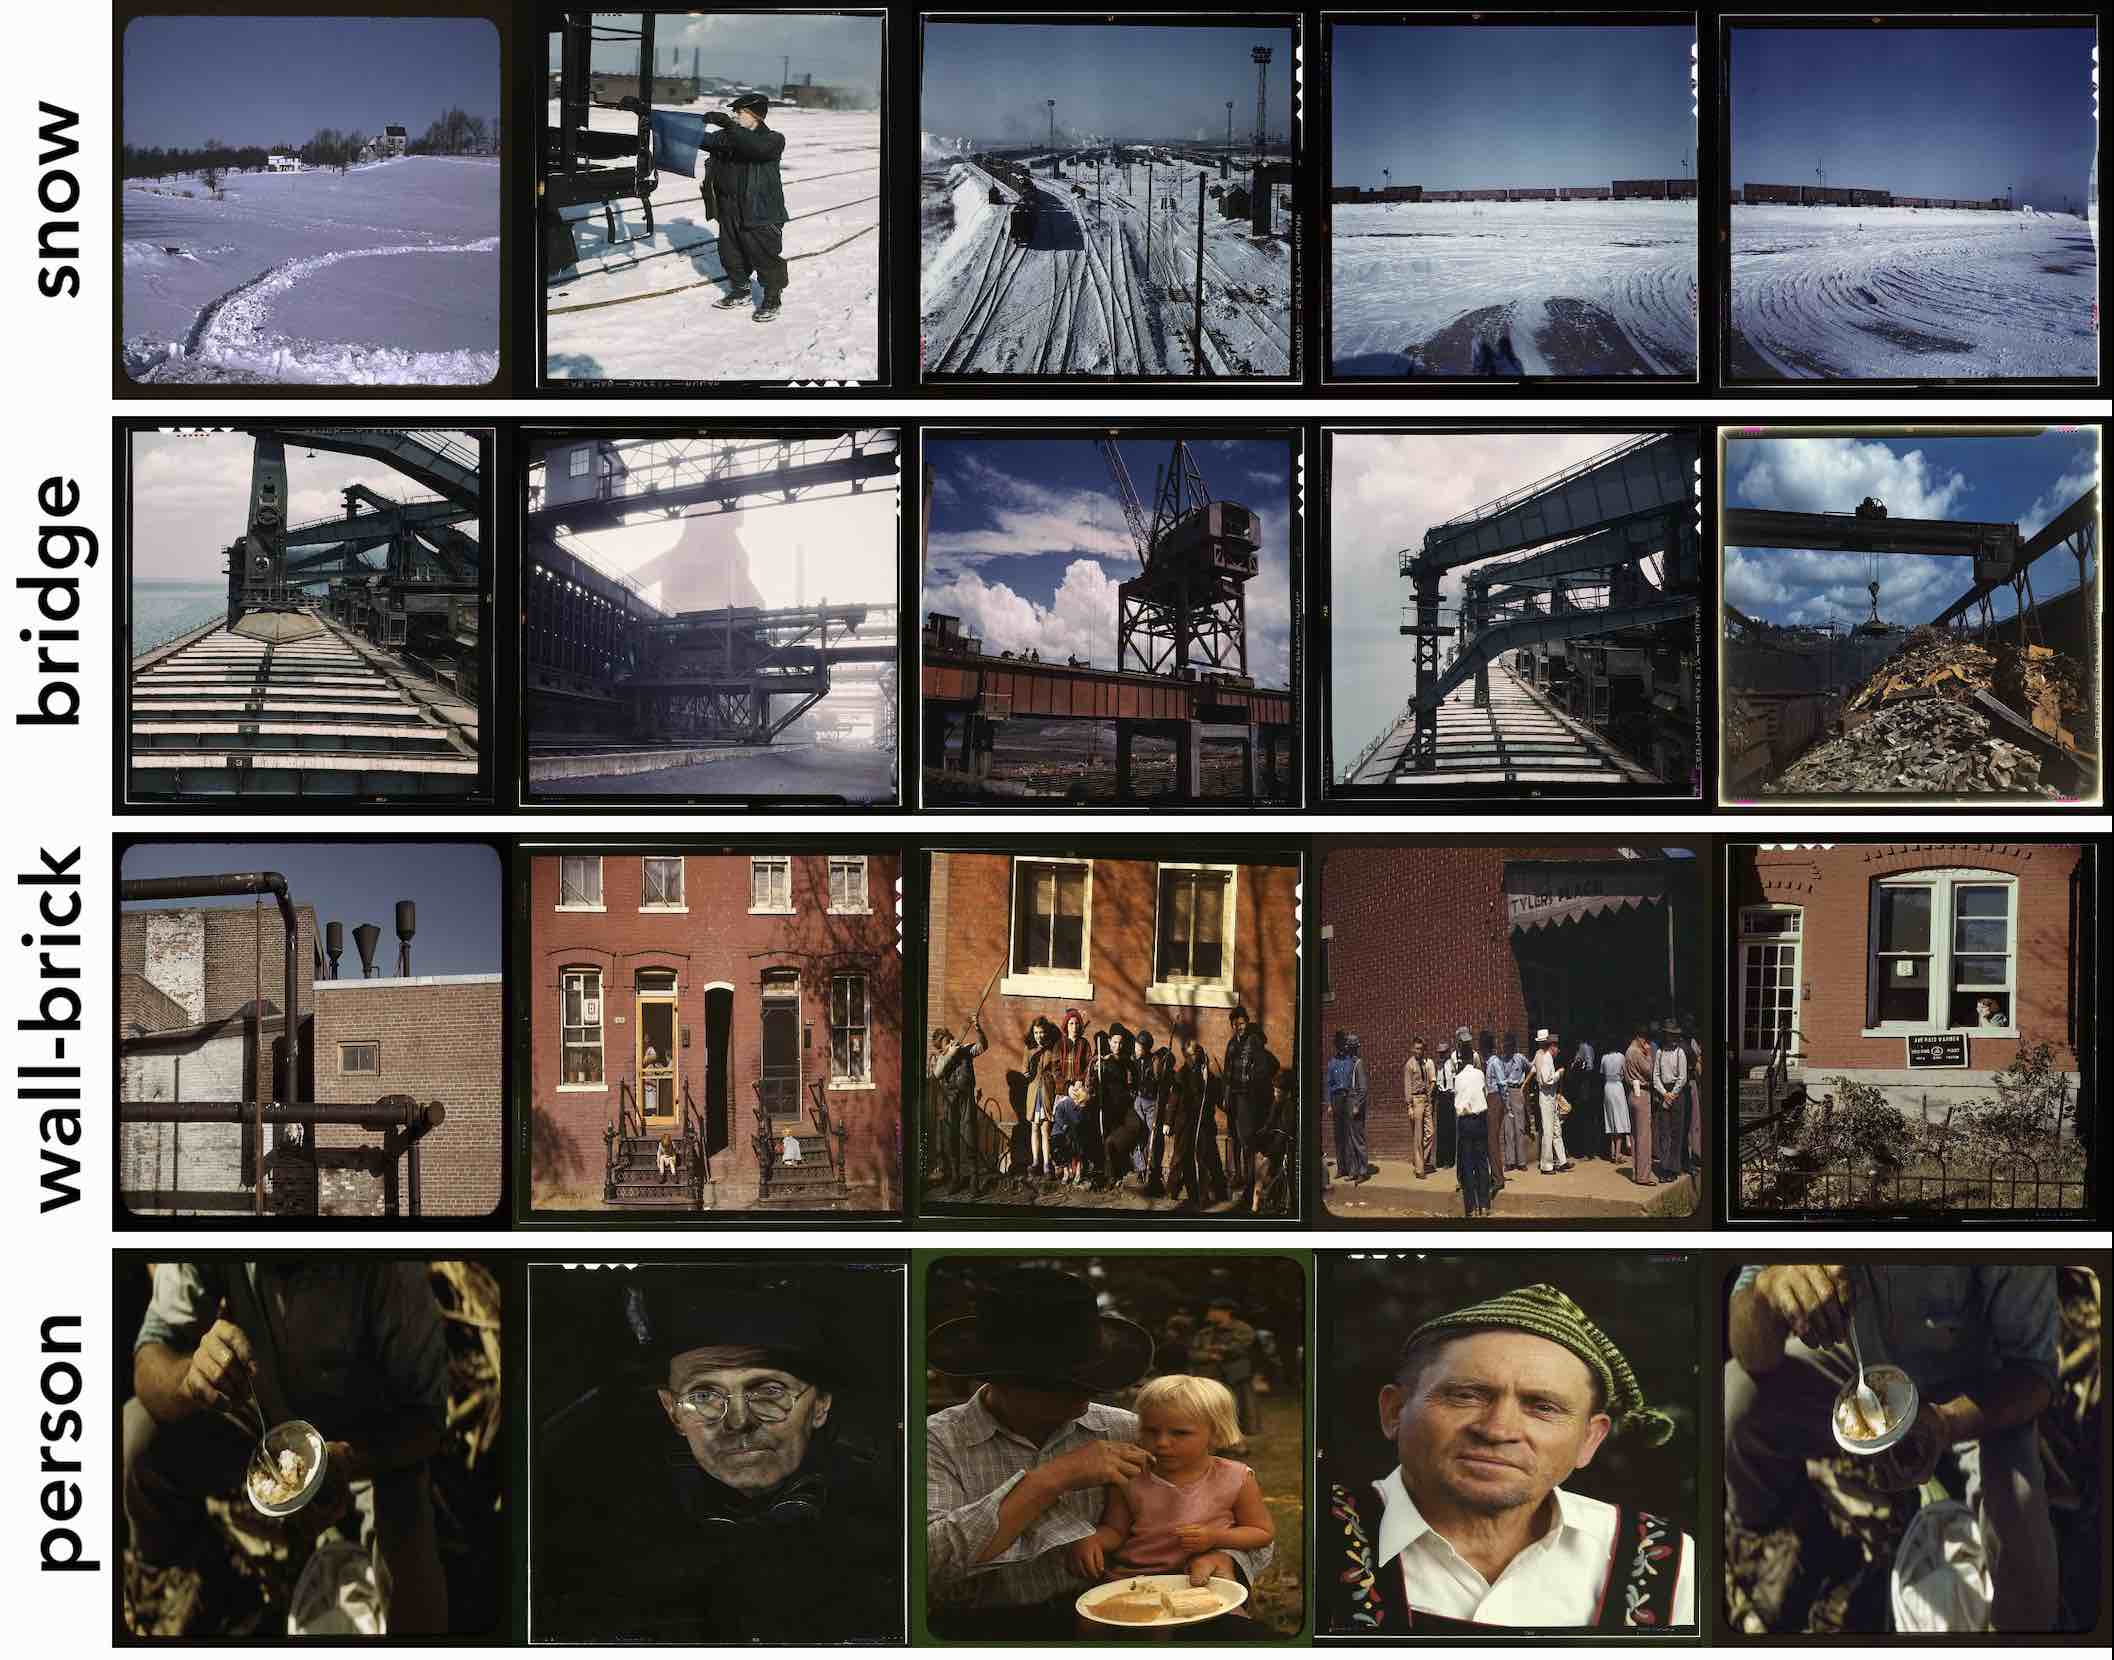
\includegraphics[width=0.95\textwidth]{../figures/max_category_grid_labels_top.jpg}
\end{center}

\end{frame}

%%%%%%%%%%%%%%%%%%%%%%%%%%%%%%%%%%%%%%%%%%%%%%%%%%%
\begin{frame}{}

\begin{center}
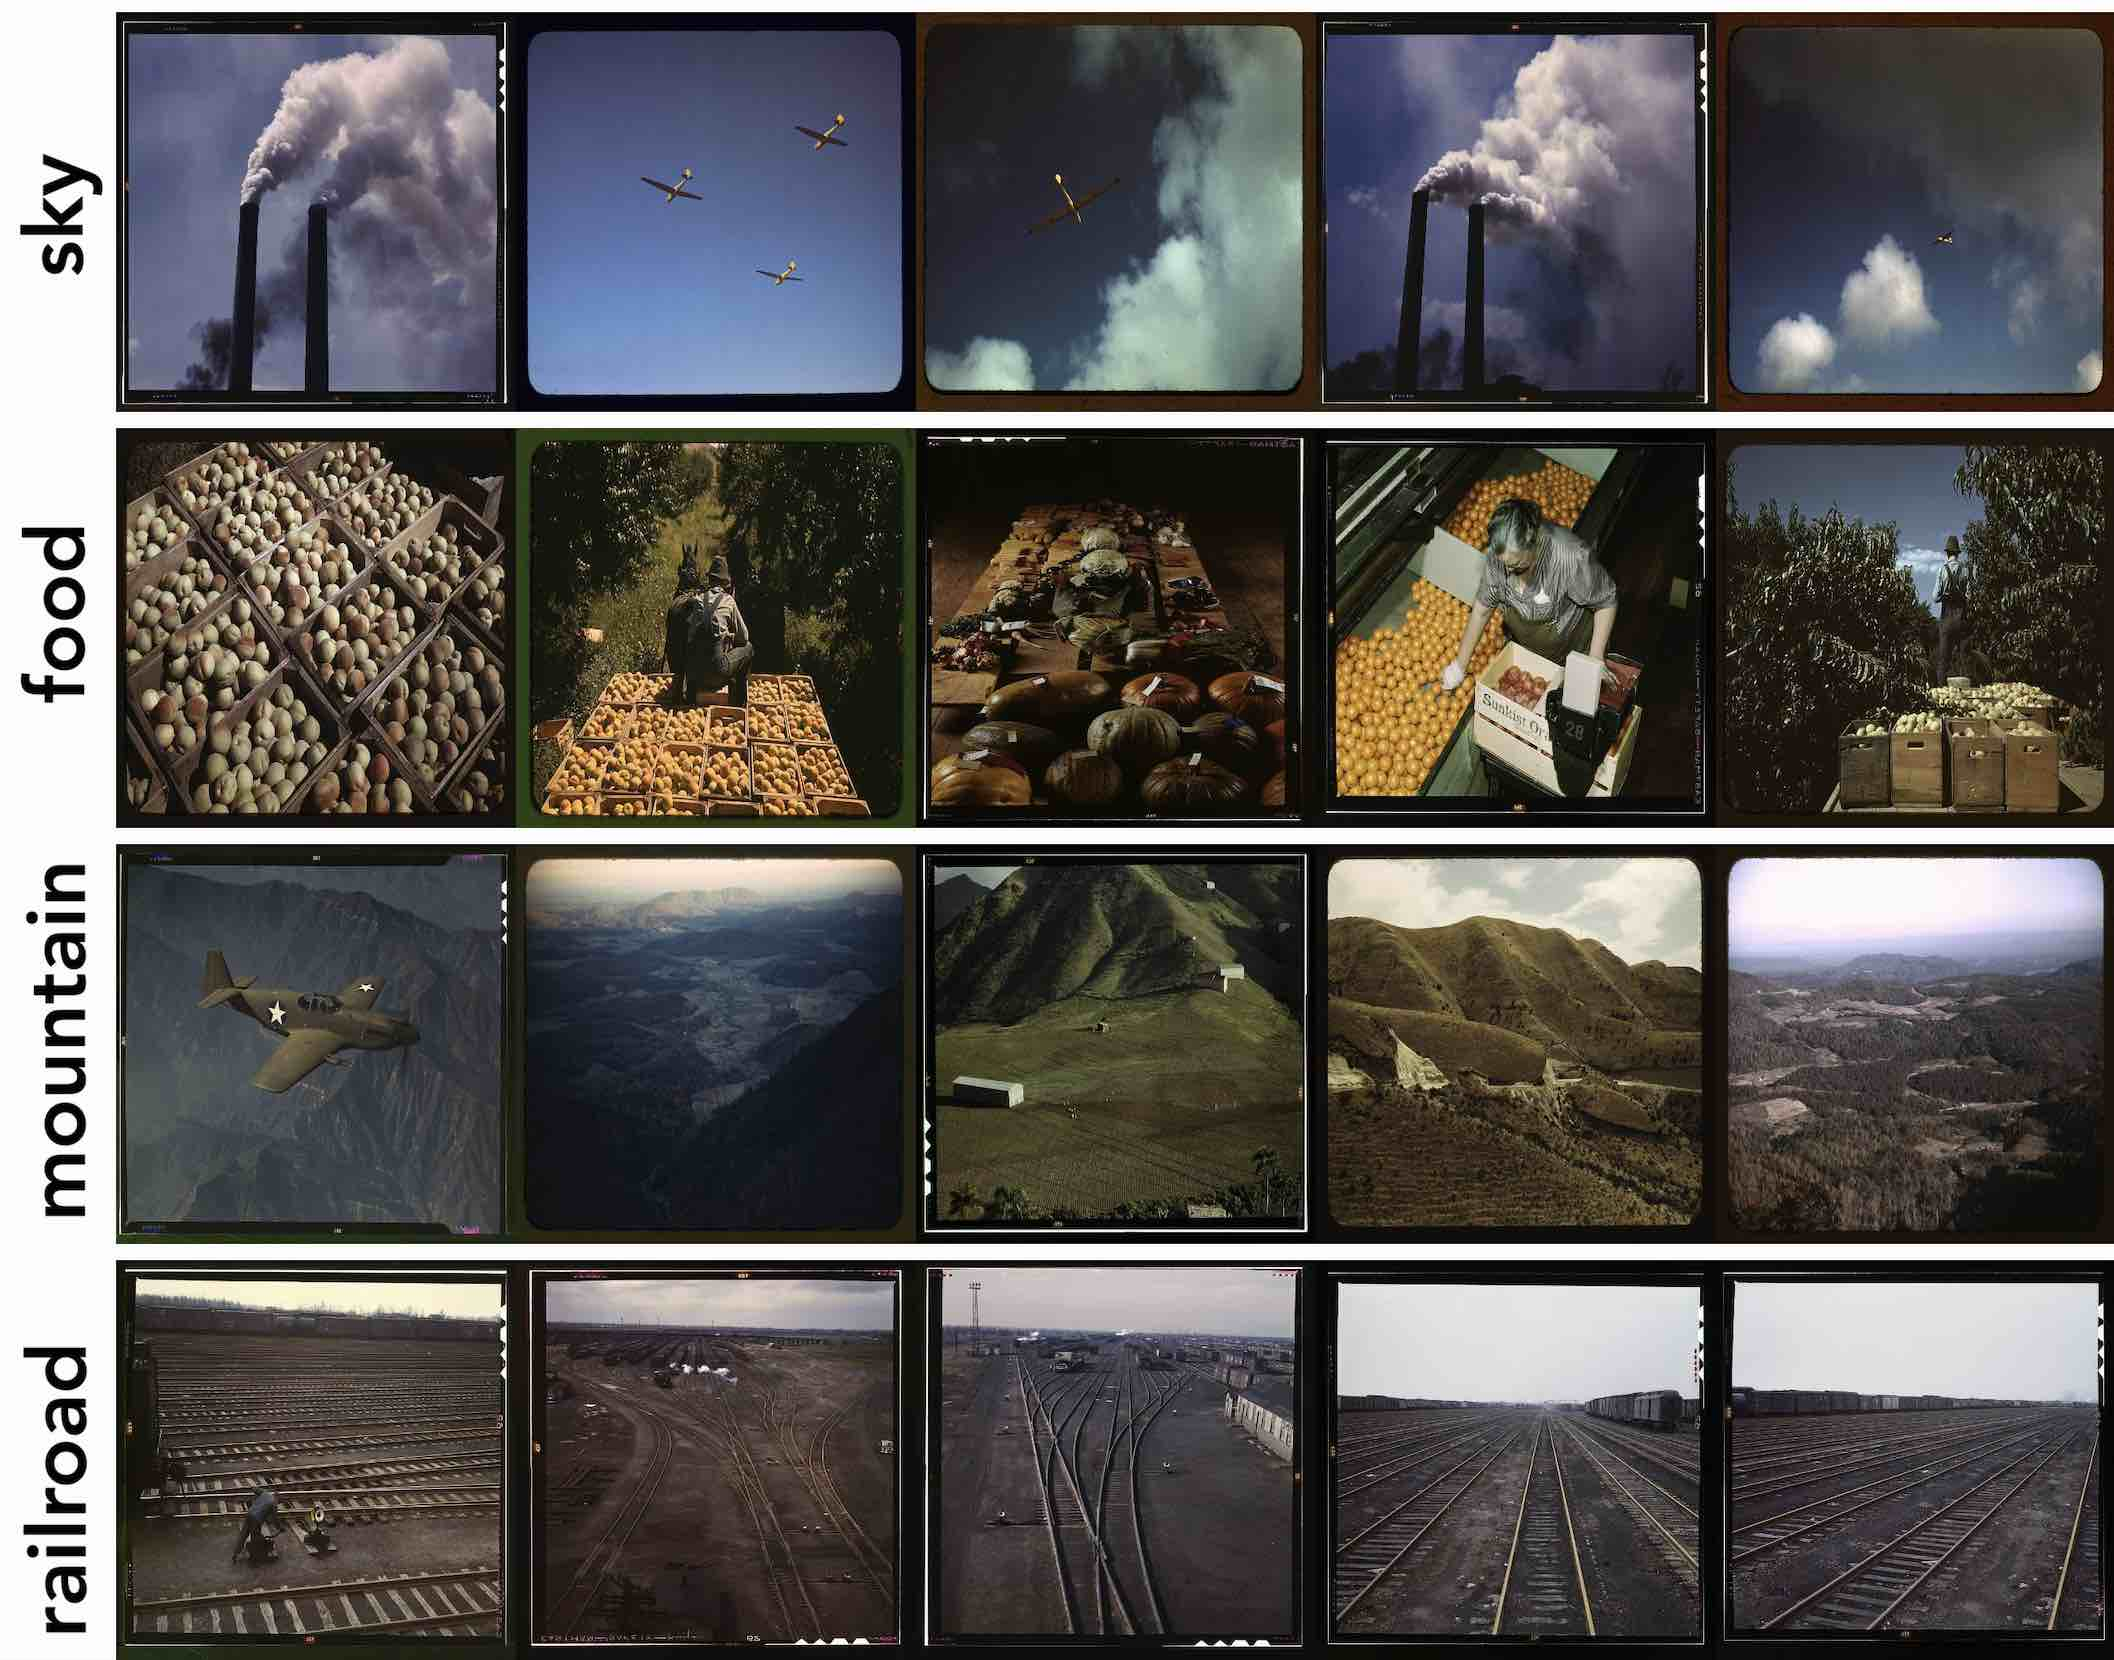
\includegraphics[width=0.95\textwidth]{../figures/max_category_grid_labels_bottom.jpg}
\end{center}

\end{frame}

%%%%%%%%%%%%%%%%%%%%%%%%%%%%%%%%%%%%%%%%%%%%%%%%%%%
\section{Evaluation}

\begin{frame}{Quantitative evaluation}
\centering

Hand labelled accuracy of the annotations generated by each method.

\begin{tabular}{lccc}
 \hline
 & \textbf{Accuracy} & \textbf{Images Labelled} & \textbf{Unique Results} \\
 \hline
Captions & 31.5\% & 100\% & 1040 \\
Objects & 70.7\% & 37.3\% & 178 \\
Stuff \& People & 97.5\% & 98.9\% & 1140 \\
  \hline
\end{tabular}

\end{frame}

%%%%%%%%%%%%%%%%%%%%%%%%%%%%%%%%%%%%%%%%%%%%%%%%%%%
\section{Future Directions}

%%%%%%%%%%%%%%%%%%%%%%%%%%%%%%%%%%%%%%%%%%%%%%%%%%%
\begin{frame}{Future Directions}

\begin{itemize}
\item further encode information about the detected
regions \textrightarrow{} dominant colors of each region type; describe regions by quadrant
\item develop a structured language for creating image captions from the structured
data
\item hierarchical version of a tagged object detection algorithm that simulates
the stuff-based regions
\end{itemize}

\end{frame}





\end{document}
